% !TEX root = ../thesis.tex
%
\chapter{Generation Learning in Computer Games}
\label{sec:analysis}

\begin{enumerate}
	\item What was measured: fitness development within neats generations 
	\item two different games: marI/O and flappy
	\item different challenges within the game
	\item 
\end{enumerate}

	\section{MarI/O}
		\label{sec:analysis:mario}
		
		\todo{screenshot of simulations}
		
		\begin{enumerate}
			\item explanation of environment and expectations
			\item fitnessfunction, formlar? when was goal reached
			\item explanation of graph of population (10, 50, 250 [why those numbers]) averaged on generations (30 generations evenly choosen [equal spaces between generation numbers] for boxplot but not for best genome)  (abstract explanation)
			\item average run counts (lines of output) per population class and in total.
			\item Differences and similarities between runs 
			\item in general summarize these three calculated values
			\item Avg fitness increase of each pop number compared to avg distance 
			\item run 250 most uniform results
		\end{enumerate}
		
		\paragraph{Population 10 / Generation 500}
			\label{par:mario10}
%			\begin{figure}[h]
%				\centering
%				\begin{minipage}{0.33\textwidth}
%					\centering
%					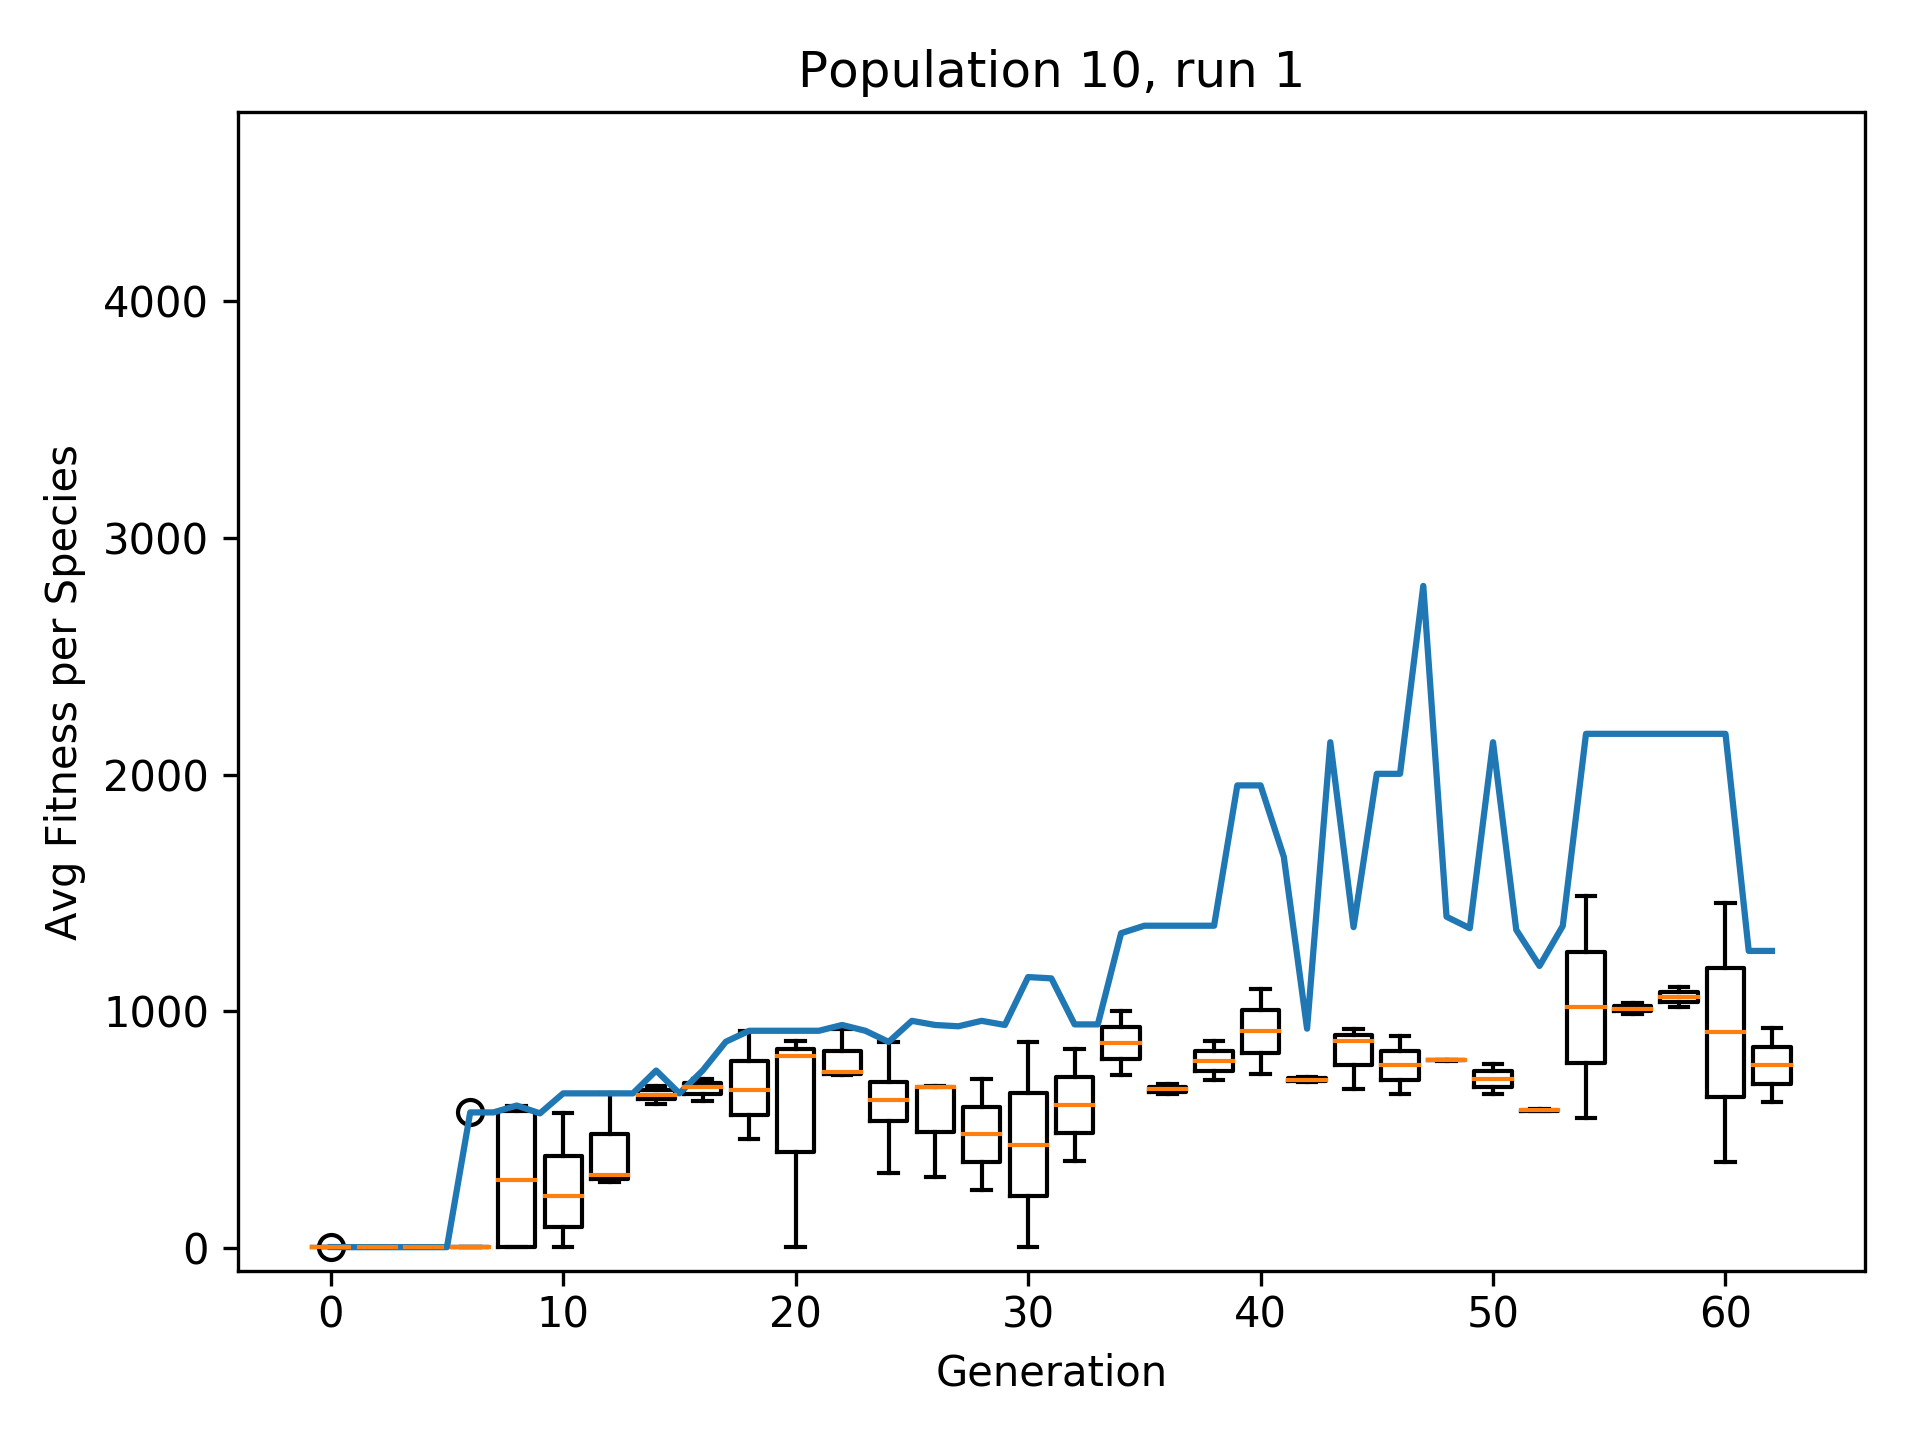
\includegraphics[width=1\textwidth]{graphics/mario/pop10_run1} % first figure itself
%				\end{minipage}\hfill
%				\begin{minipage}{0.33\textwidth}
%					\centering
%					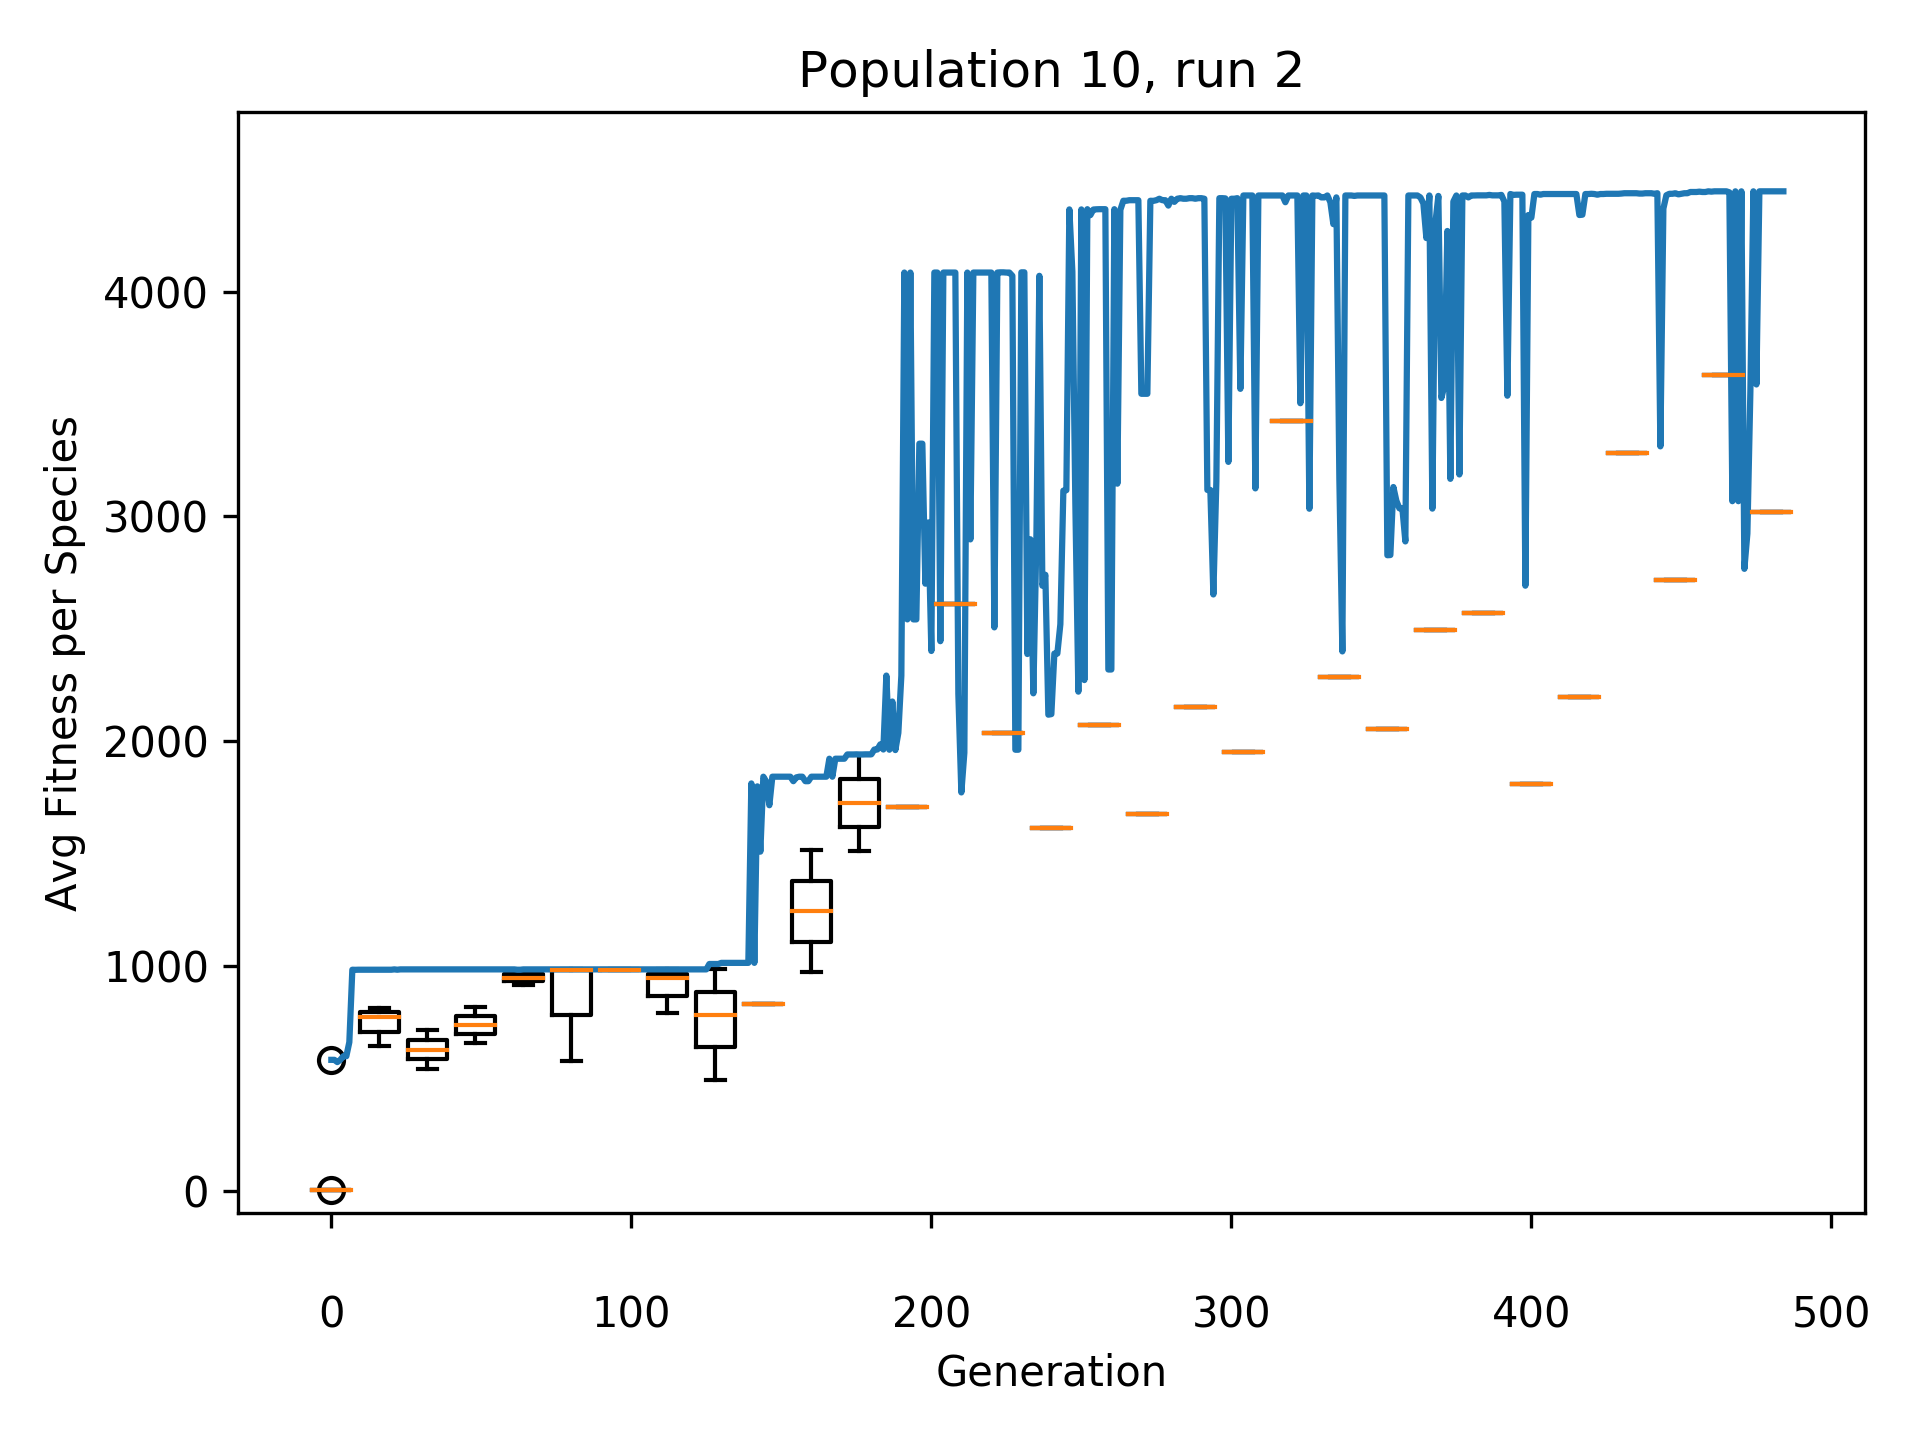
\includegraphics[width=1\textwidth]{graphics/mario/pop10_run2} % second figure itself
%				\end{minipage}
%				\begin{minipage}{0.33\textwidth}
%					\centering
%					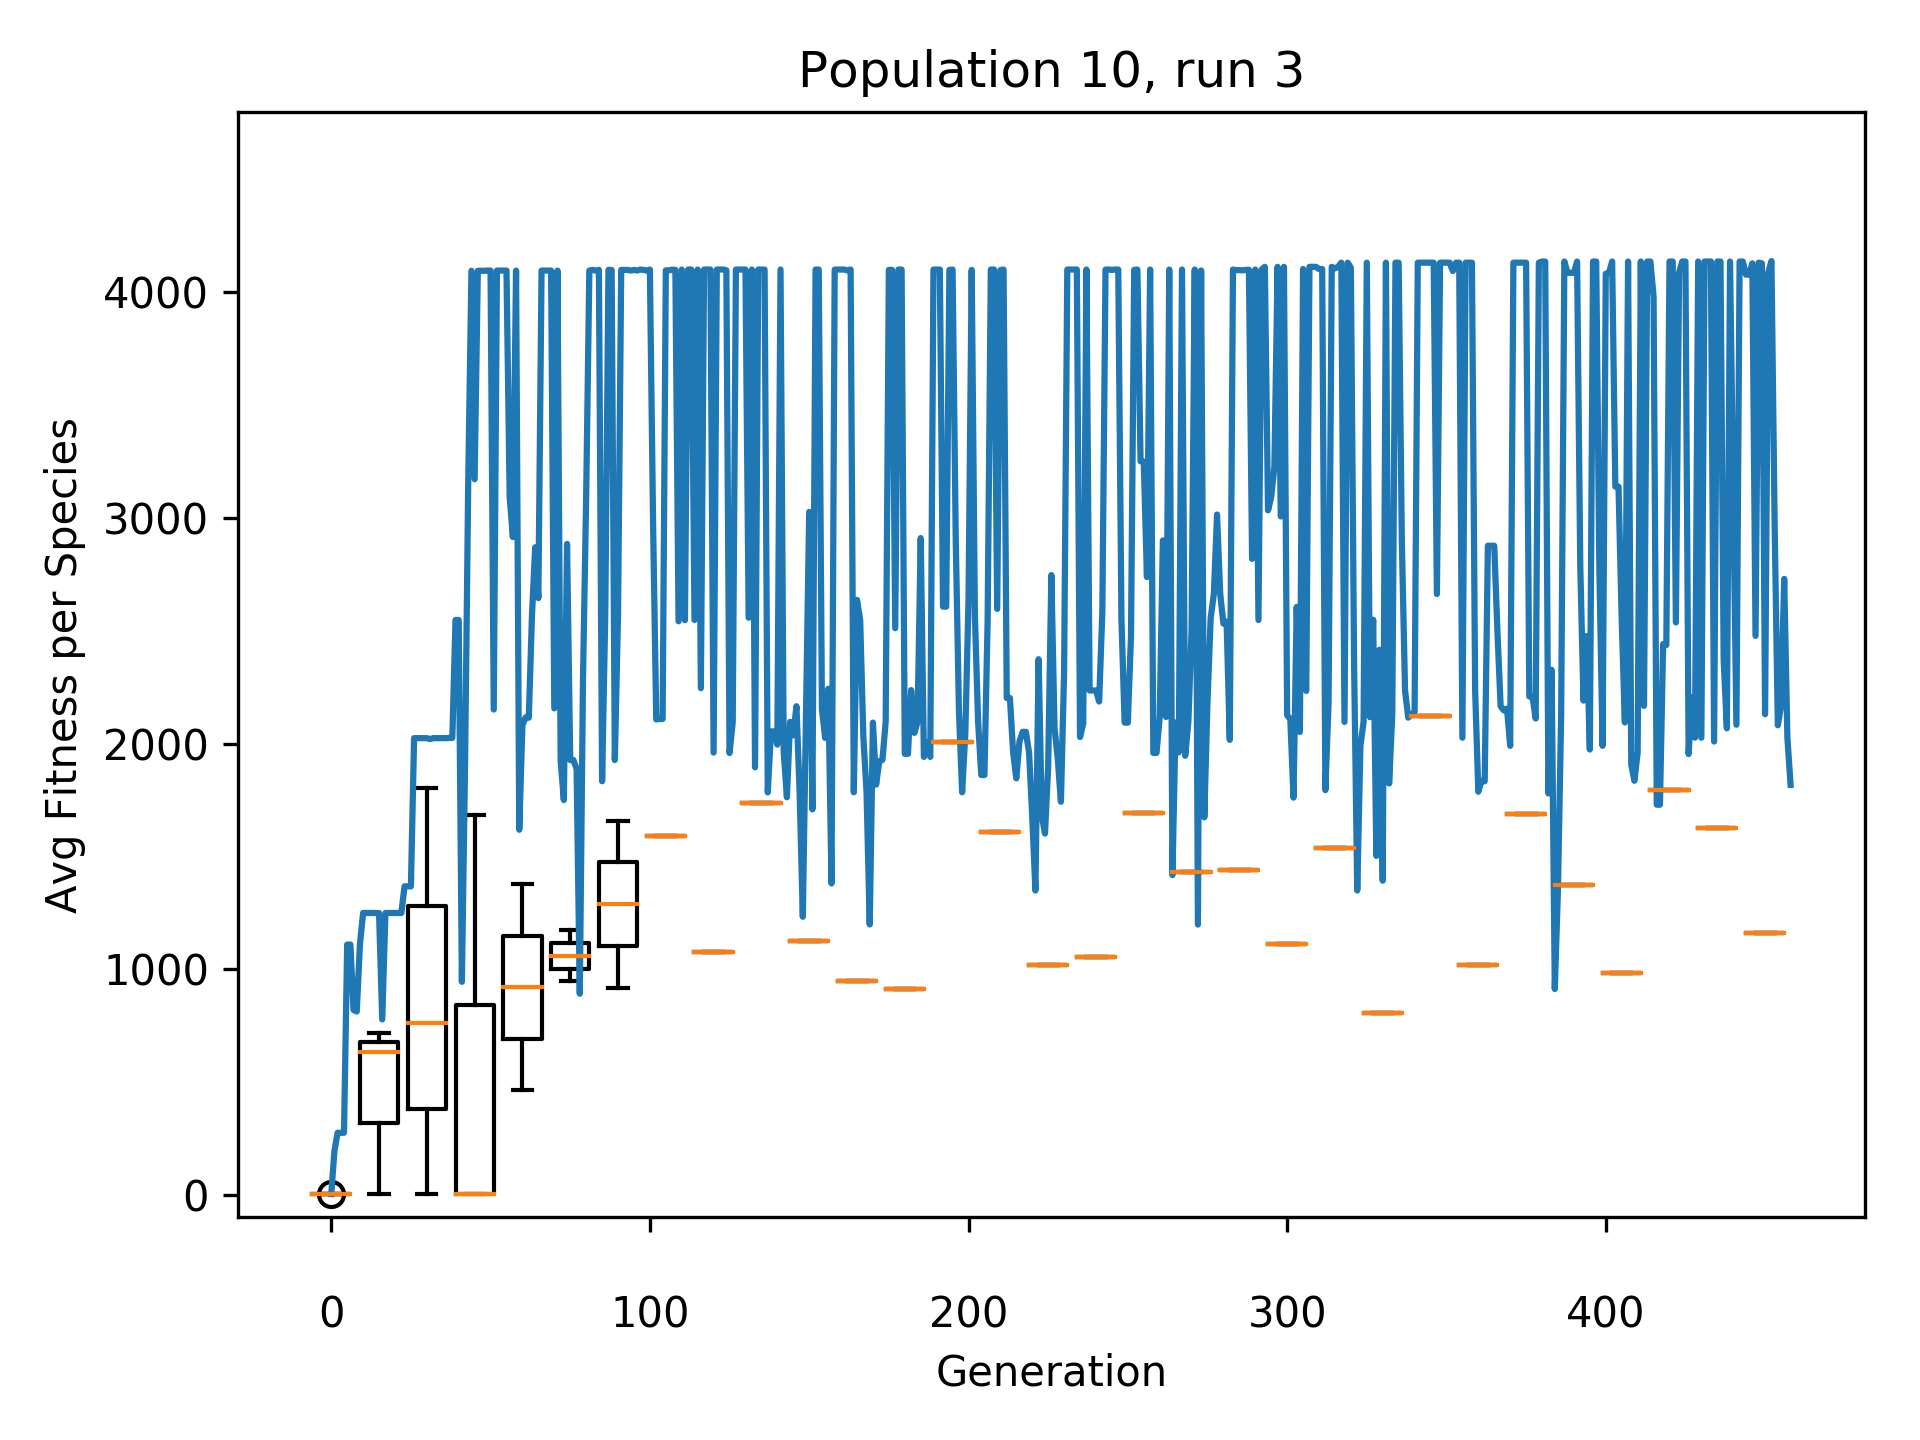
\includegraphics[width=1\textwidth]{graphics/mario/pop10_run3} % second figure itself
%				\end{minipage}
%				\caption{MarI/O Population 10}
%				\label{fig:mario10}
%			\end{figure}
			As it is visible in Figure \ref{fig:mario10} the vertical axis shows the fitness score average of the genomes within a species. The horizontal axis portrays the generations containing the species. Each generation contains up to 10 populations which is divided into species and genomes within species. This species devision was made based on the NEAT algorithm described in section \ref{sec:related:neat}. The best run of the genomes grouped by each generation is marked with a blue line. Therefore the blue line indicates the best overall run within a generation. Since the boxplot portrays the species's avarage score of each generation and the the blue line shows the best run per genome (population), the boxplot and the blue line rarely meet. Still the average population score is closer to the best run than in the next two population variants (see later in this section population 50 \ref{par:mario50} and population 250 \ref{par:mario250}). This can be calculated by taking the median of the species fitnesses and substracting that number from the best run of the genomes:
			$average\_distance = \frac{\sum\nolimits_{g_i \in generations} max(g_i.genomes) - median(g_i.species)}{|generations|}\approx1107$ whereas $g_i.genomes$ and $g_i.species$ are lists of the respective fitnesses. \\
			In the three runs on average $334.\overline{6}$ generations were created which results in a skipping of generations inside the graphics of around $11.1\overline{5}$ generations averagely between two displayed generations. Unfortunately the first run crashed after generation 60. Still, because of the long runtime of the simulation the run was kept. However, indicated by plot run 2 and 3, the population growth started after this generation. As it can be seen in the 3rd run of the figure \ref{fig:mario10}, sometimes runs over 3000 fitness score could be achieved even after the 30th generation. In run 2 the average fitness of the species tend to rise, however more and longer runs would be needed to test this hypothesis.\\
			In each generations there are up to 10 populations. \todo{(up to because of neat implementation check neat implementation}
			In the first generation (Gen 0) no mating was done, so in the first generation there where 10 species spawned with one genome each. In the 10th Generation on average only $4.\overline{3}$ species where left. After generation 50 maximum 3 species where left in all runs and after generation 190 in run 2 and after generation 91 in run 3, respectively, only 1 species was left for mating. The mating results into the corssover of species.\\
			All runs except plot run 1 reached the goal (the end of the level) multiple times which can be seen by the fitnesscore being over 4000. However plot run 3 reached the goal the earliest with runs over 4096 starting from generation 44. Still there was the most overall regress made in plot run 3. This can be calculated by adding the differences between the best runs of each generation if the difference was negative: $average\_regress = \frac{\sum\nolimits_{g_i \in generations} min(max(g_i.genomes) - max(g_{i-1}.genomes), 0)}{|generations|}\approx-348$ again whereas $g_i.genomes$ is a list of the fitnesses of each genome inside the generation. The regress of plot-run 1 was $-88.27$ approximately and of plot-run 2 was around $-109.98$.\\
			In plot run 1 the $average\_fitness\_increase =  \frac{\sum\nolimits_{g_i \in generations} max(g_i.genomes) - max(g_{i-1}.genomes)}{|generations|}\approx19.87$ was the biggest of the three runs since run 1 ended early and run 3 had many drawbacks. The average fitness increase of run 2 was around $7.97$ and of run 3 was only $3.95$ approximately. Since it is only slightly possible to extend the maximum score above the score of 4000 and run 1 has never reached this ranking, run 1 pointed out to have the best score increase per round. Every successful round, whereas Mario reached the goal will only minimize the fitness increase when averaged with the generation count. In another words, for an infinitely large amount of generations the $average\_fitness\_increase$ is expected to converge to $0$ since the game has and end-state in contrast to the game Flappy Bird, as it can be seen in section \ref{sec:analysis:flappy}. In mathematical terms: $\lim\limits_{n \to \infty} average\_fitness\_increase(n) = 0$, whereas the $average\_fitness\_increase(n)$ is defined as the average fitness increase of a set of n generations.
			
			\begin{enumerate}
				\item there are up to 10 populations in each generation (up to because of neat implementation \todo{check neat implementation})
				\item Differences similarities between runs
			\end{enumerate}
		
		\paragraph{Population 50 / Generation 100}
			\label{par:mario50}
			\begin{figure}[h]
				\centering
				\begin{minipage}{0.33\textwidth}
					\centering
					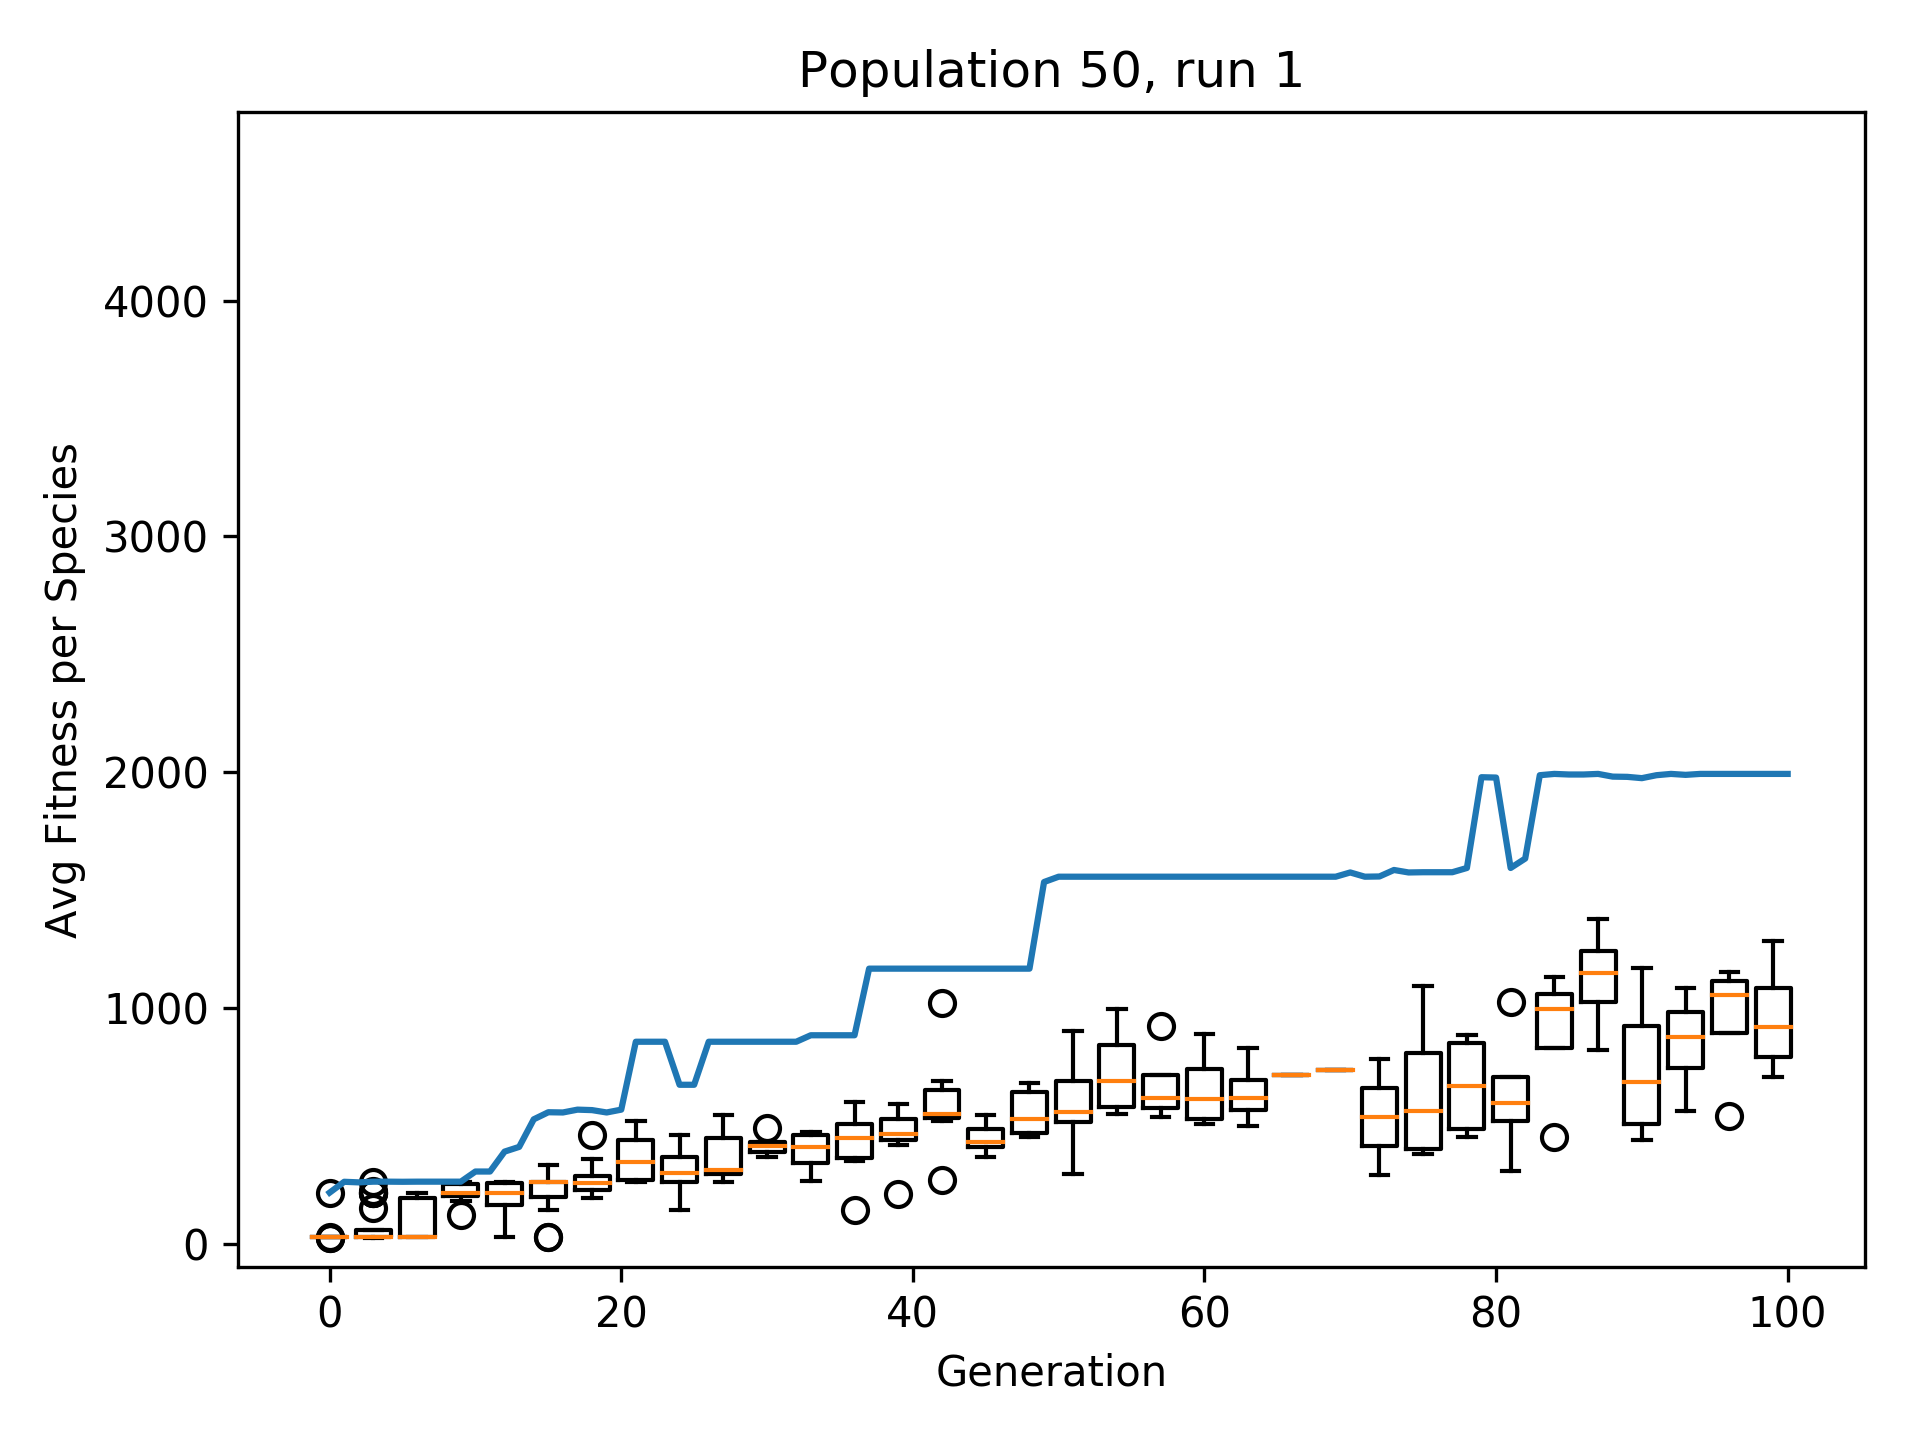
\includegraphics[width=1\textwidth]{graphics/mario/pop50_run1} % first figure itself
				\end{minipage}\hfill
				\begin{minipage}{0.33\textwidth}
					\centering
					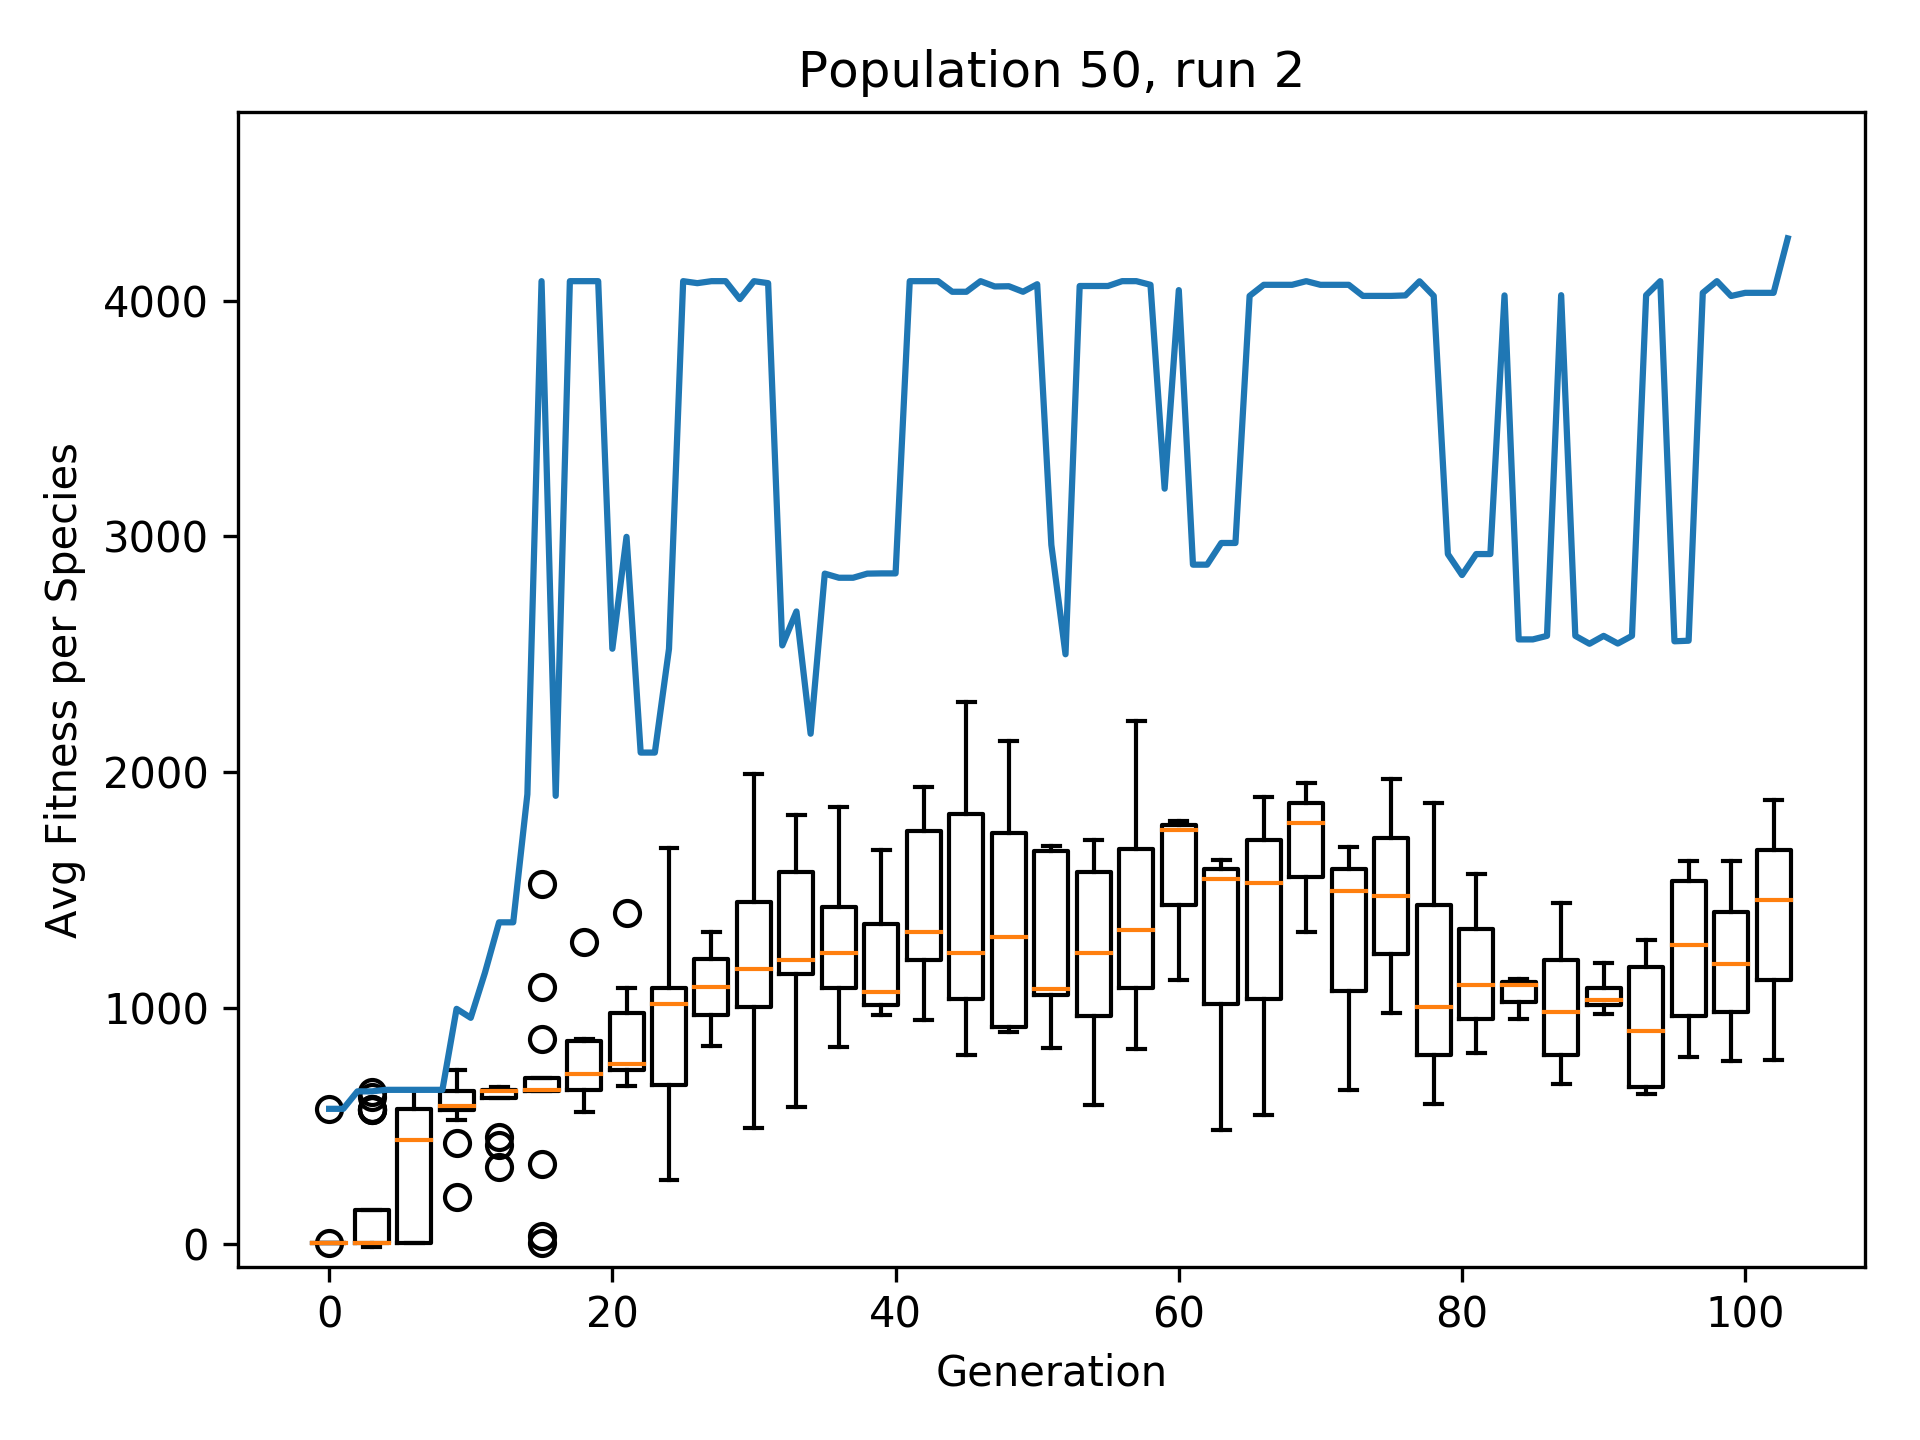
\includegraphics[width=1\textwidth]{graphics/mario/pop50_run2} % second figure itself
				\end{minipage}
				\begin{minipage}{0.33\textwidth}
					\centering
					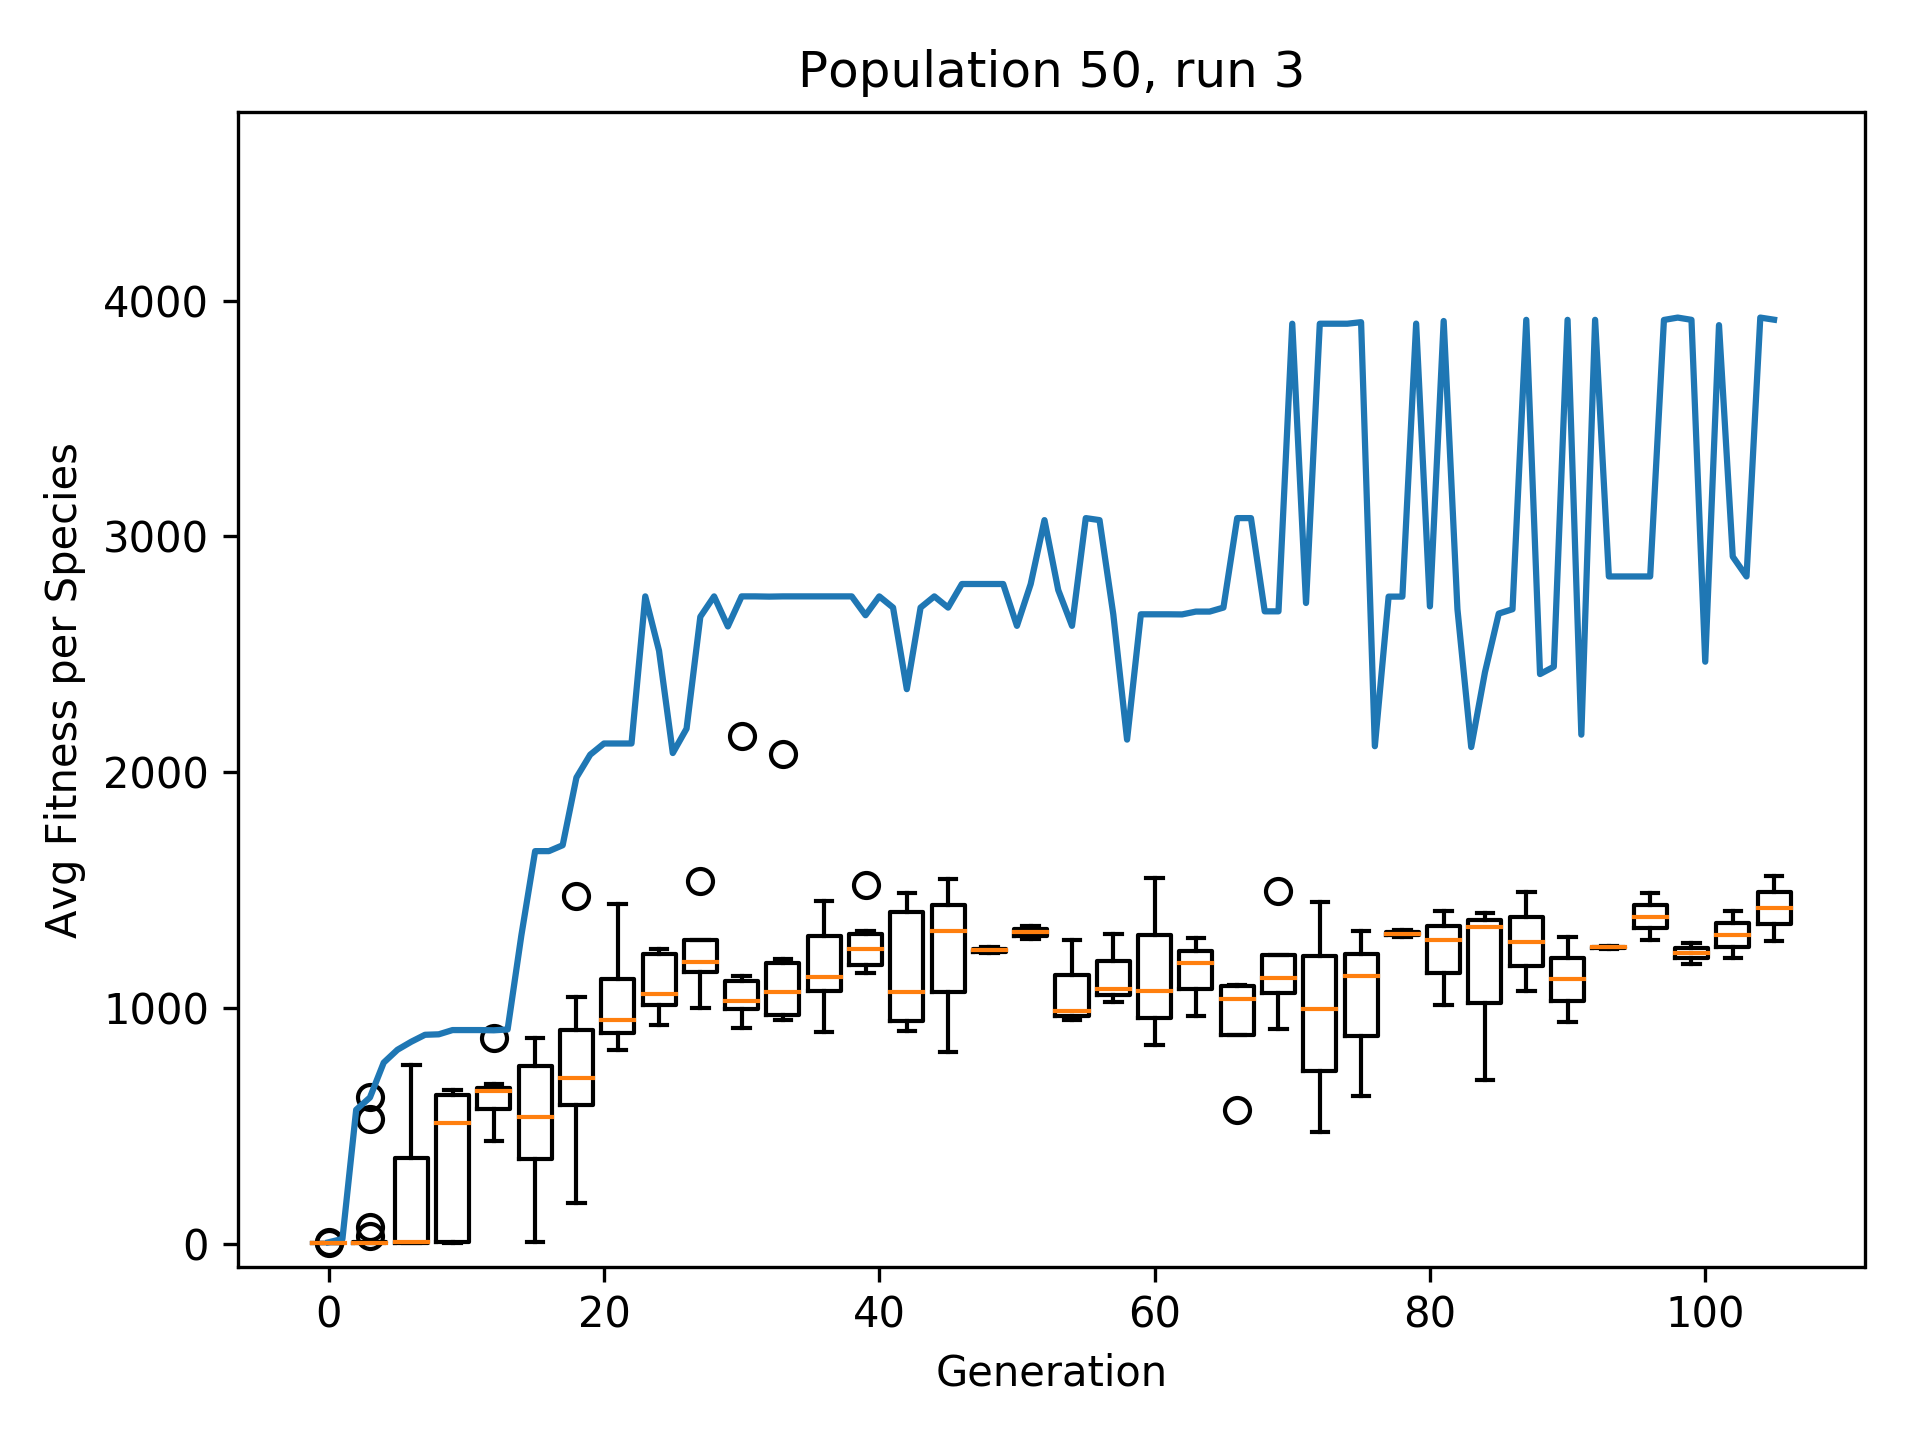
\includegraphics[width=1\textwidth]{graphics/mario/pop50_run3} % second figure itself
				\end{minipage}
				\caption{MarI/O Population 50}
				\label{fig:mario50}
			\end{figure}
			In this setup the population count is up to 50, again distributed into species and genomes within species according to the MarI/O NEAT implementation. The $average\_distance$  between the median of the species of each generation to the best genome run of this generation is bigger than that of the simulation with it's initial population size of 10 but it is smaller than in the last case. The $average\_distance$ was calculated as described in the previous simulation (population 10 \ref{par:mario10}) and the value is approximately $1406$.\\
			In this simulations the runs where executed until there where over 100 generations (101 generations in run 1, 104 in run 2 and 106 in run 3). This results in an average skipping of 3.456 generations between the display of two generations.\\
			In generation 0 there where 50 species spawned, again, with one genome each. In the 10th generation there where 15 species left on average. At the end of generation 100 on average $3.\overline{3}$ species where left from the initial 50 generations.\\
			Interestingly the plot run 1 couldn't learn to reach the goal. From this data it is not trivial to predict if the breakthrough would have started within the next 50 generations or if this run would have stayed low in it's fitness score, since there are no clear patterns to find in the graphical representation of these runs. In order to answer on this question more profoundly, further and longer runs have to be made and the big jumps between the fitness scores of each neighbour generation would have to be analysed.\\
			Plot run 2 and 3 had more luck in reaching the end, however run 3 had more stability in it's high score results between generations. Still after generation 70 plot run 3 also shows stronger differences between it's generation's heigh scores. Nevertheless, plot-run 2 reached the goal the earliest. The first time run 2 acheived a fitness-score over 4000 was in generation 15 (it reached a score of $4082.5$), whereas plot-run 3 reached a maximum score of $3928$ in generation 98. Still run 3 reached to goal with a score of $3902$ the first time in generation 70. The 3rd plot-run has the highest $average\_fitness\_increase\approx36.92$ of the three runs. Plot-run 1 has an $average\_fitness\_increase$ of $17.58$ approximately and plot-run 2 of $35.5$ precisely.\\
		
		
		\paragraph{Population 250 / Generation 30}
			\label{par:mario250}
			\begin{figure}[h]
				\centering
				\begin{minipage}{0.33\textwidth}
					\centering
					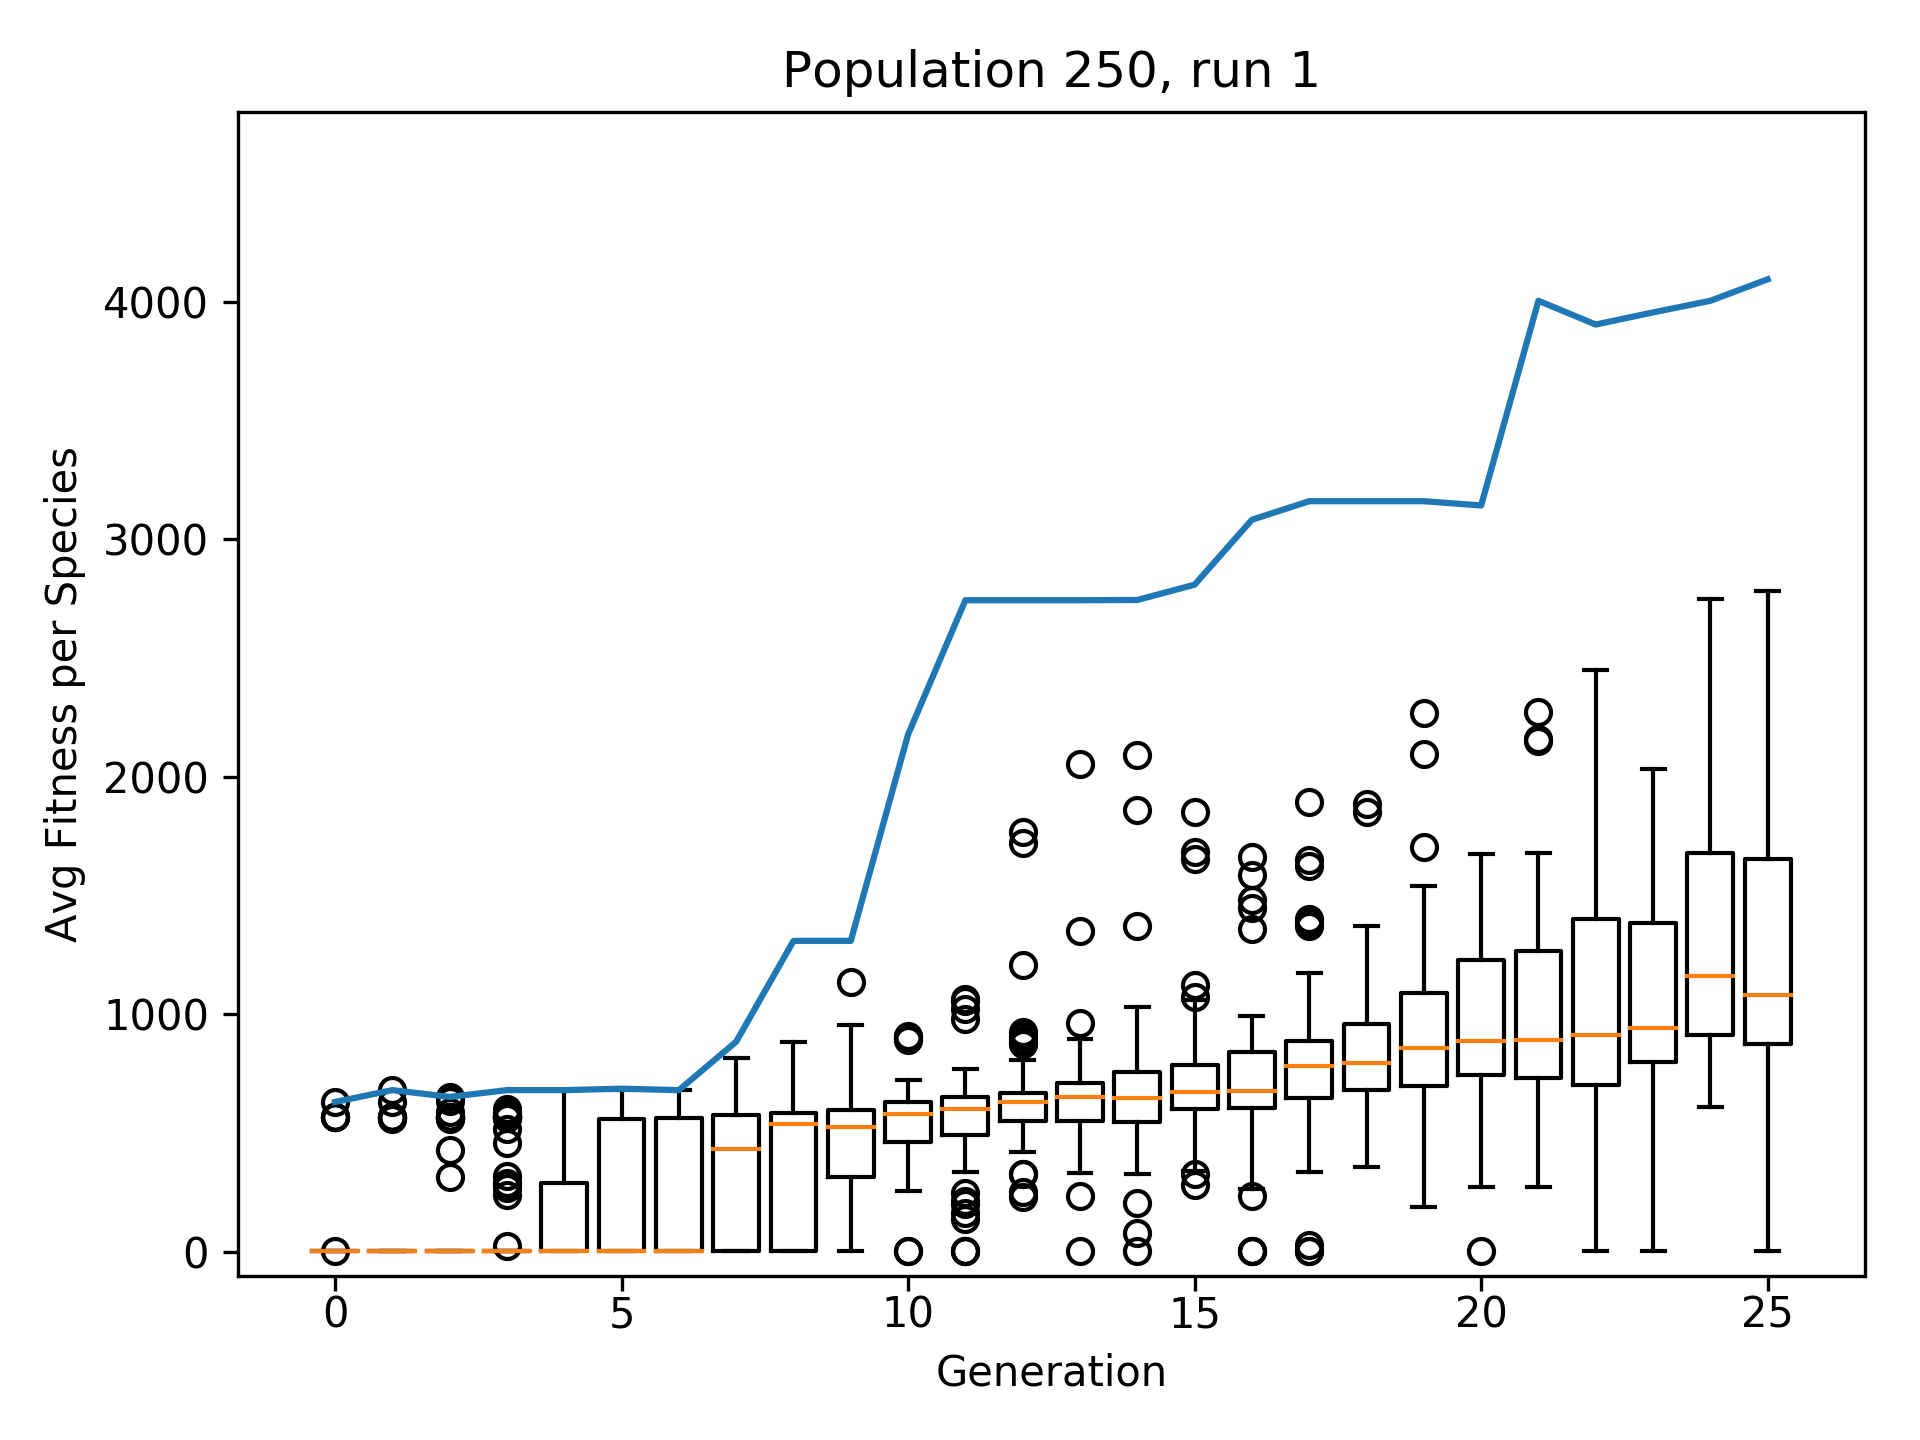
\includegraphics[width=1\textwidth]{graphics/mario/pop250_run1} % first figure itself
				\end{minipage}\hfill
				\begin{minipage}{0.33\textwidth}
					\centering
					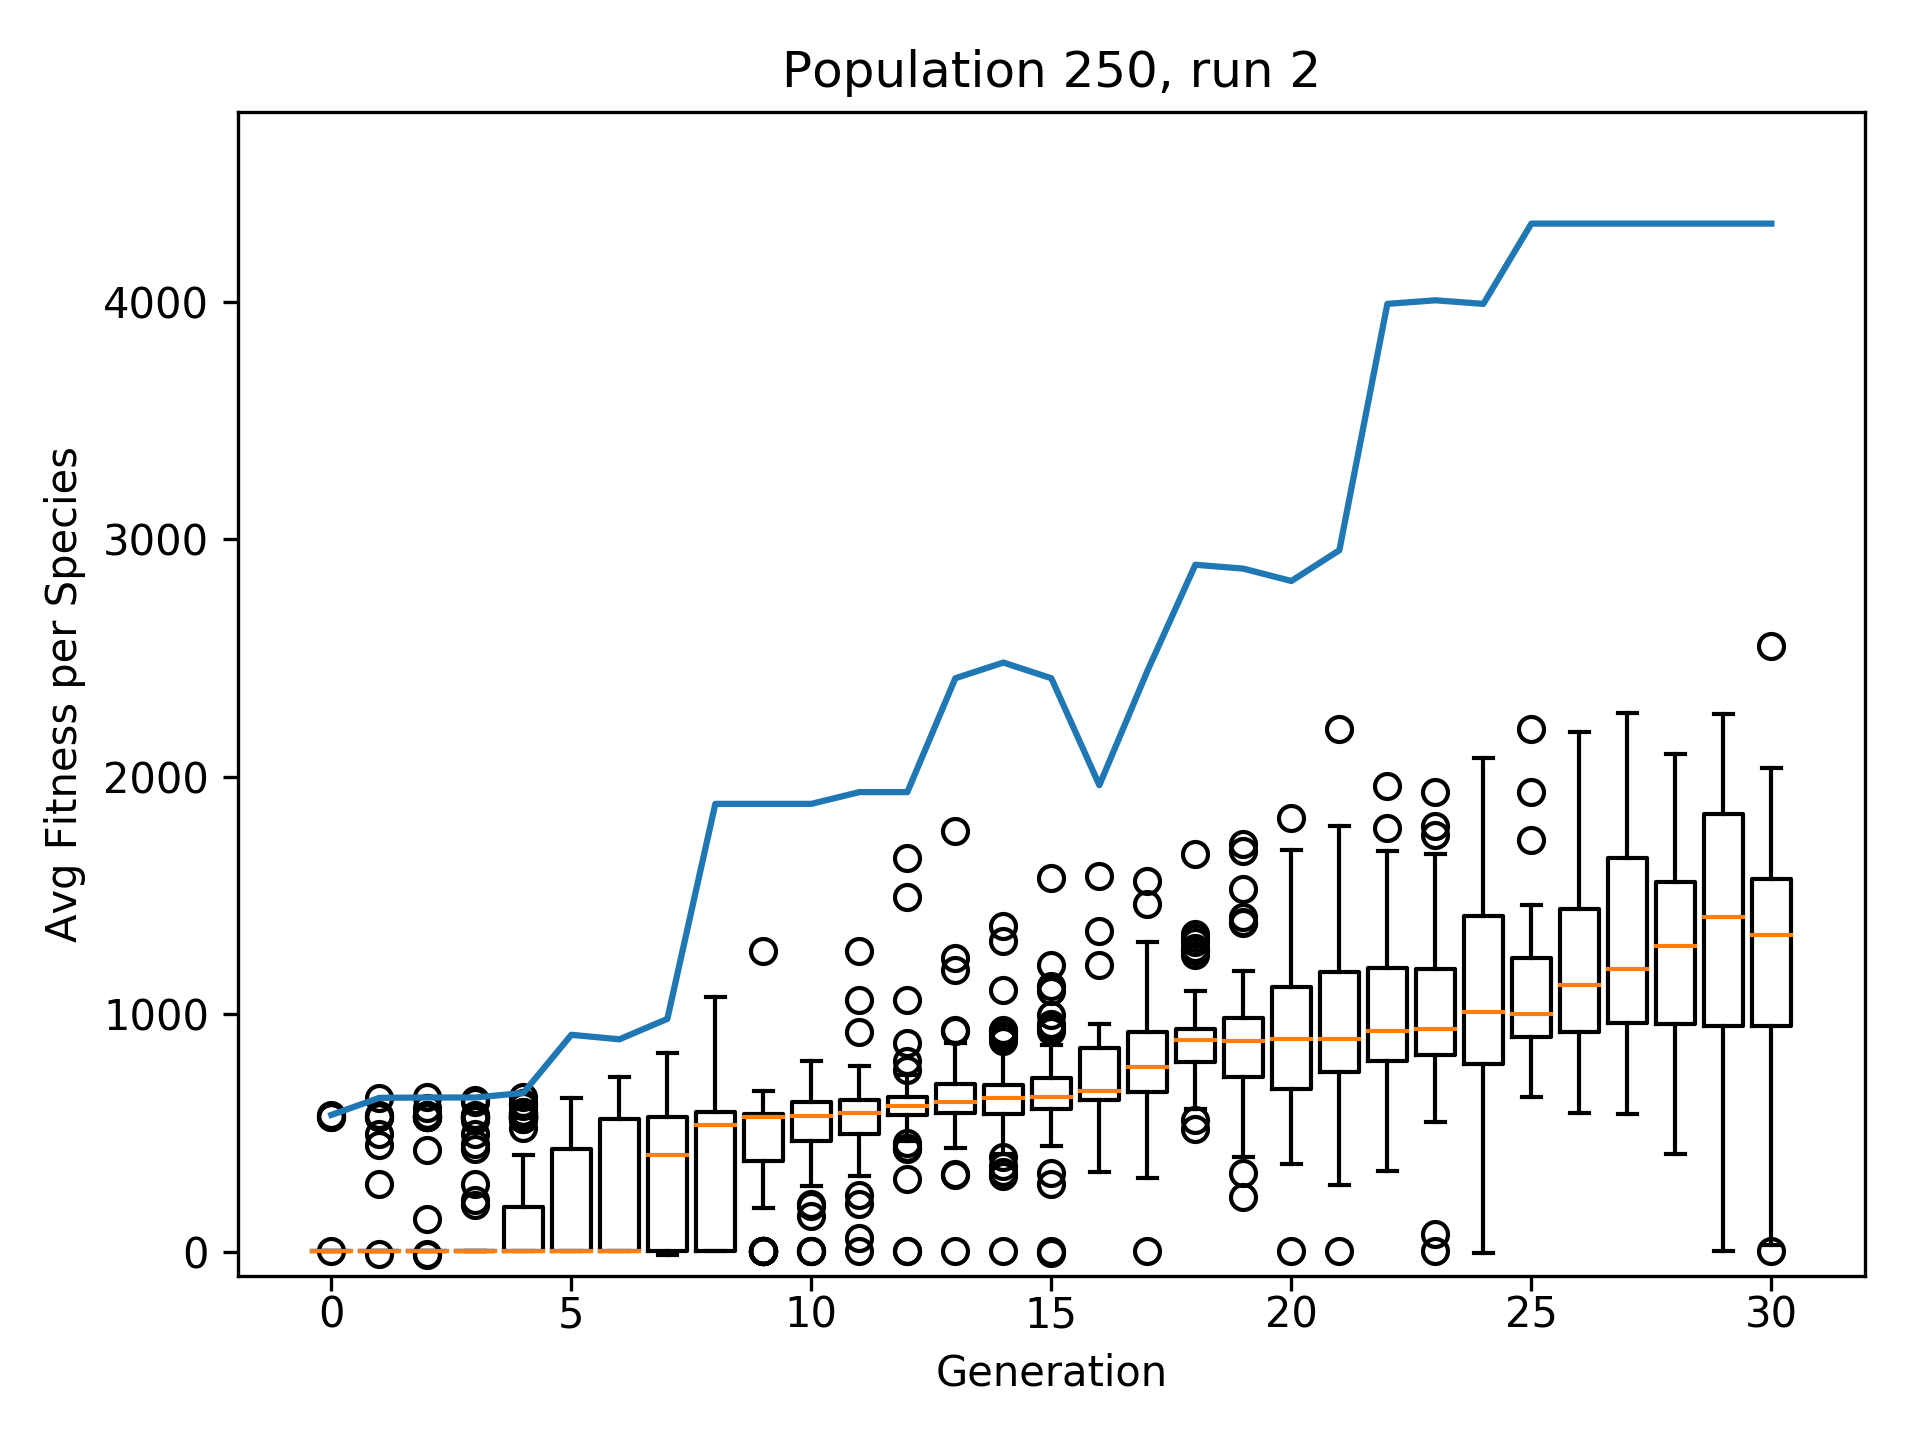
\includegraphics[width=1\textwidth]{graphics/mario/pop250_run2} % second figure itself
				\end{minipage}
				\begin{minipage}{0.33\textwidth}
					\centering
					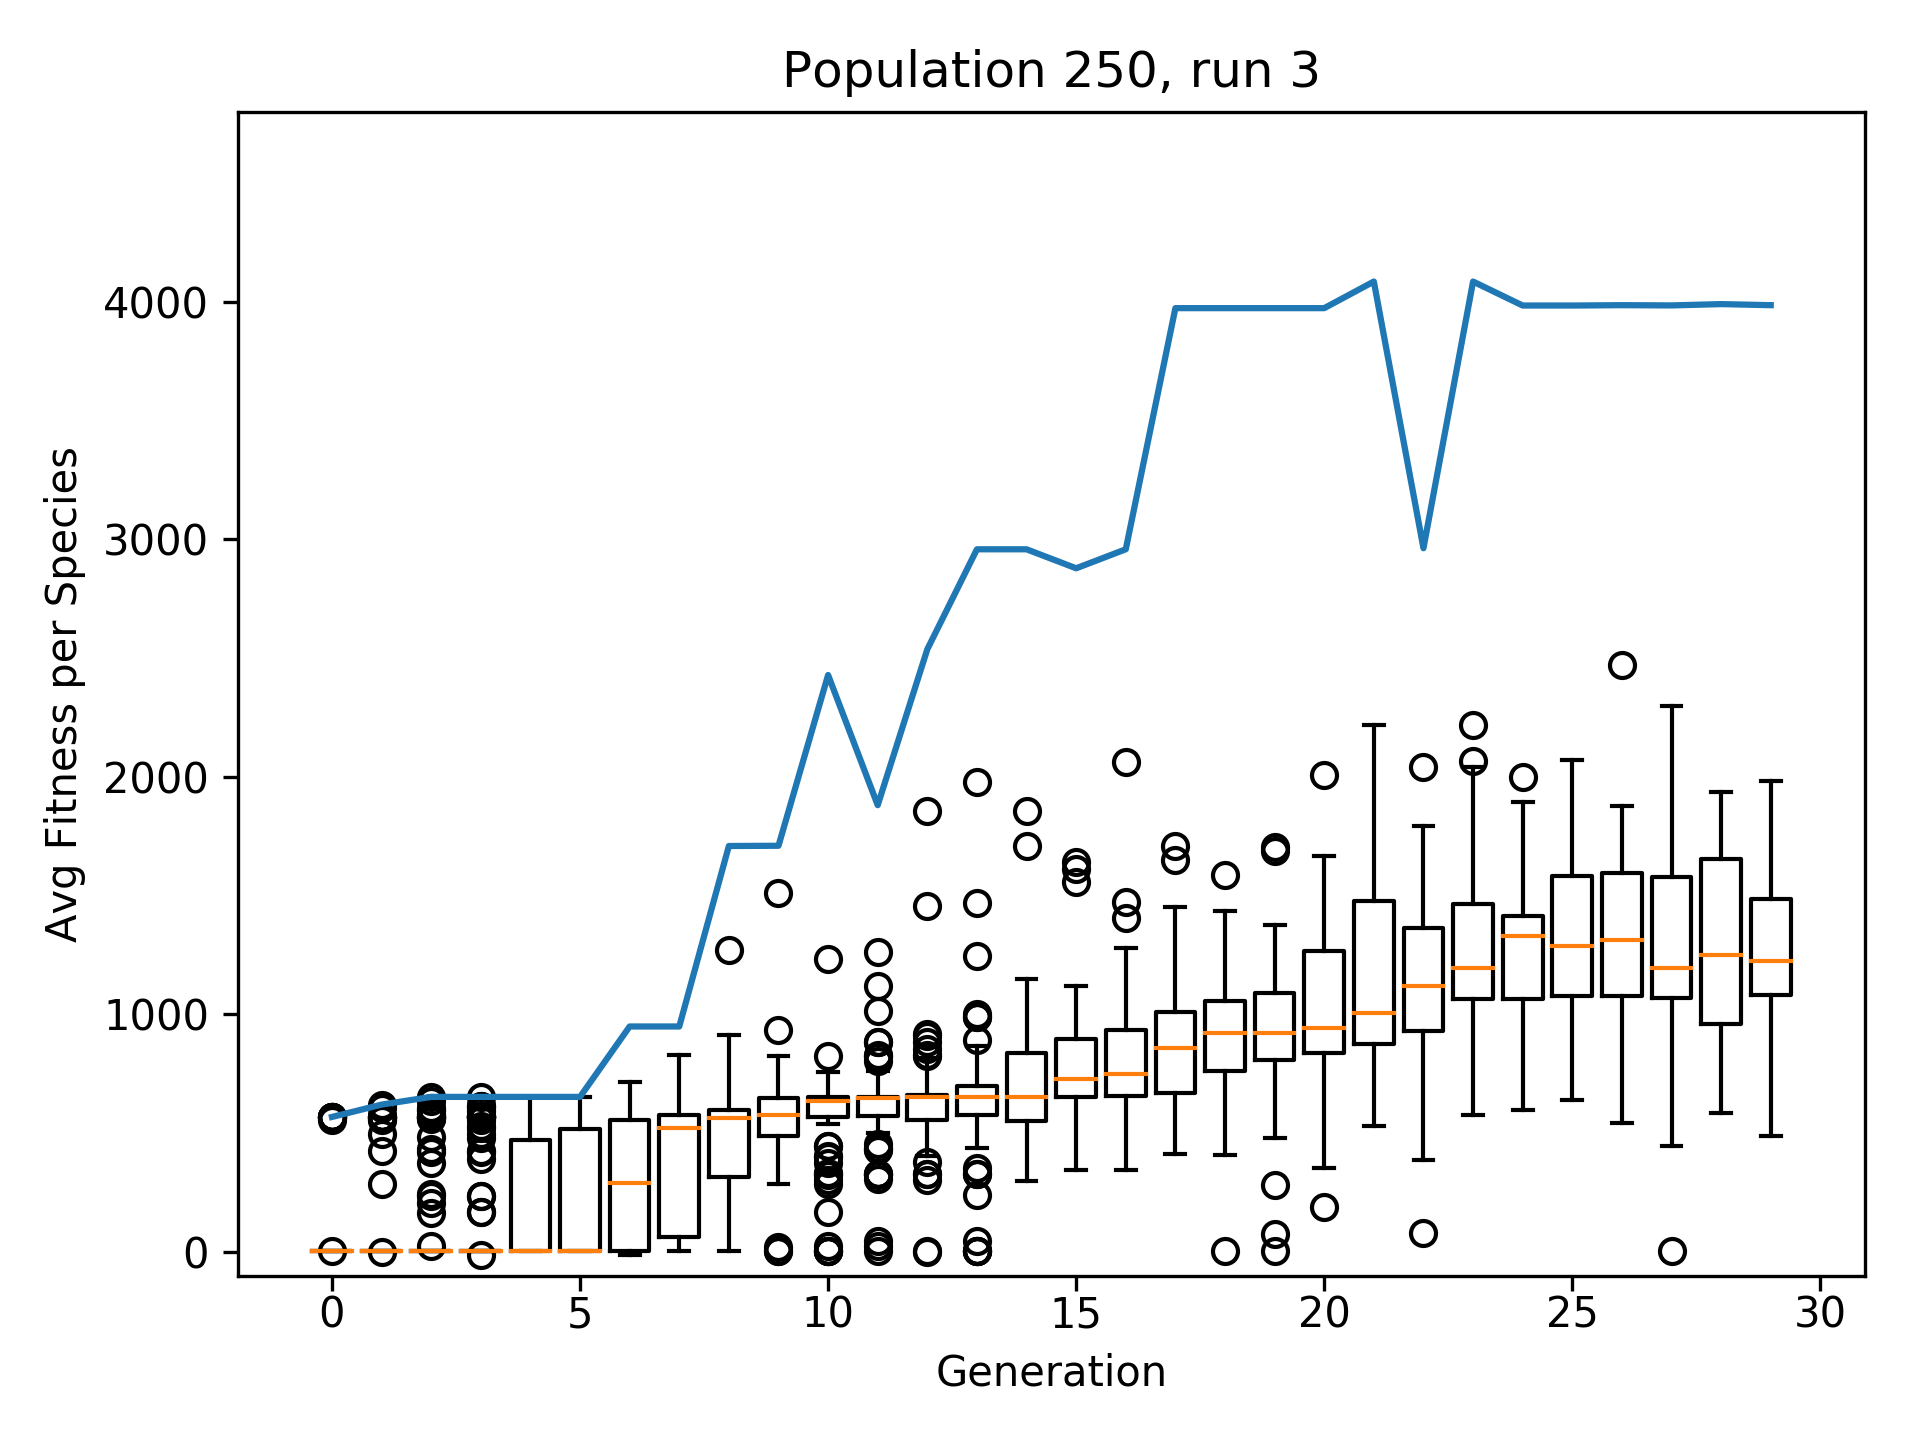
\includegraphics[width=1\textwidth]{graphics/mario/pop250_run3} % second figure itself
				\end{minipage}
				\caption{MarI/O Population 250}
				\label{fig:mario250}
			\end{figure}
			In figure \ref{fig:mario250} the population size is up to 250 in generation 0. In the first generation (Gen 0) 250 species are born with one genome each. The $average\_distance$ for this plot-runs is the biggest with approximately $1827$ when compared to the plot-runs with an initial population size of 10 and 50. In this plots no generations had to be skipped in order to portray a descriptive graph since the maximum generation count is 30 in run 2 (25 generations in run 1 and 29 generations in run 3).\\
			Already in the 6th generation, on average only 94.8 species where left. At the end of generation 25 there where 31 species left on average. \\
			Compared to the other two population classes there are at least 7 times more species left at the end of the simulations which results in longer whiskers of the boxplot.The wiskers even contains bad starts with fitness-scores lower than 100 in plot-run 1 and 2. Interestingly the best runs are always exceptions after generation 6 (in plot-run 1 and 2 even earlier). \\
			Further it is to mention that the plots are rather uniform compared to the plots of population 10 and 50. Therefore the $average\_fitness\_increase$ has similar values with a low variance which are $133.25$ for generation 1, around $121.08$ for generation 2 and $113.95$ for generation 3. The $average\_regress$ is the lowest in run 1 with $-5.87$ approximately. This is because the maximum value of the succeeding generation is smaller then the previous generation in only 4 cases. The other two plot-runs have an $average\_regress$ of approximately $-19.97$ in run 2 and $-61.92$ in run 3. All of the runs reached the end of the level even thought run 3 reached the end at generation 17, whereas plot-run 1 reached the end at generation 23 and plot-run 2 at generation 22.	
	
	% FLAPPY BIRD ###############################################################
	
	\section{Machine Learning Flappy Bird}
		\label{sec:analysis:flappy}
		\todo{change this title}
		
		\begin{figure}[h]
			\centering
			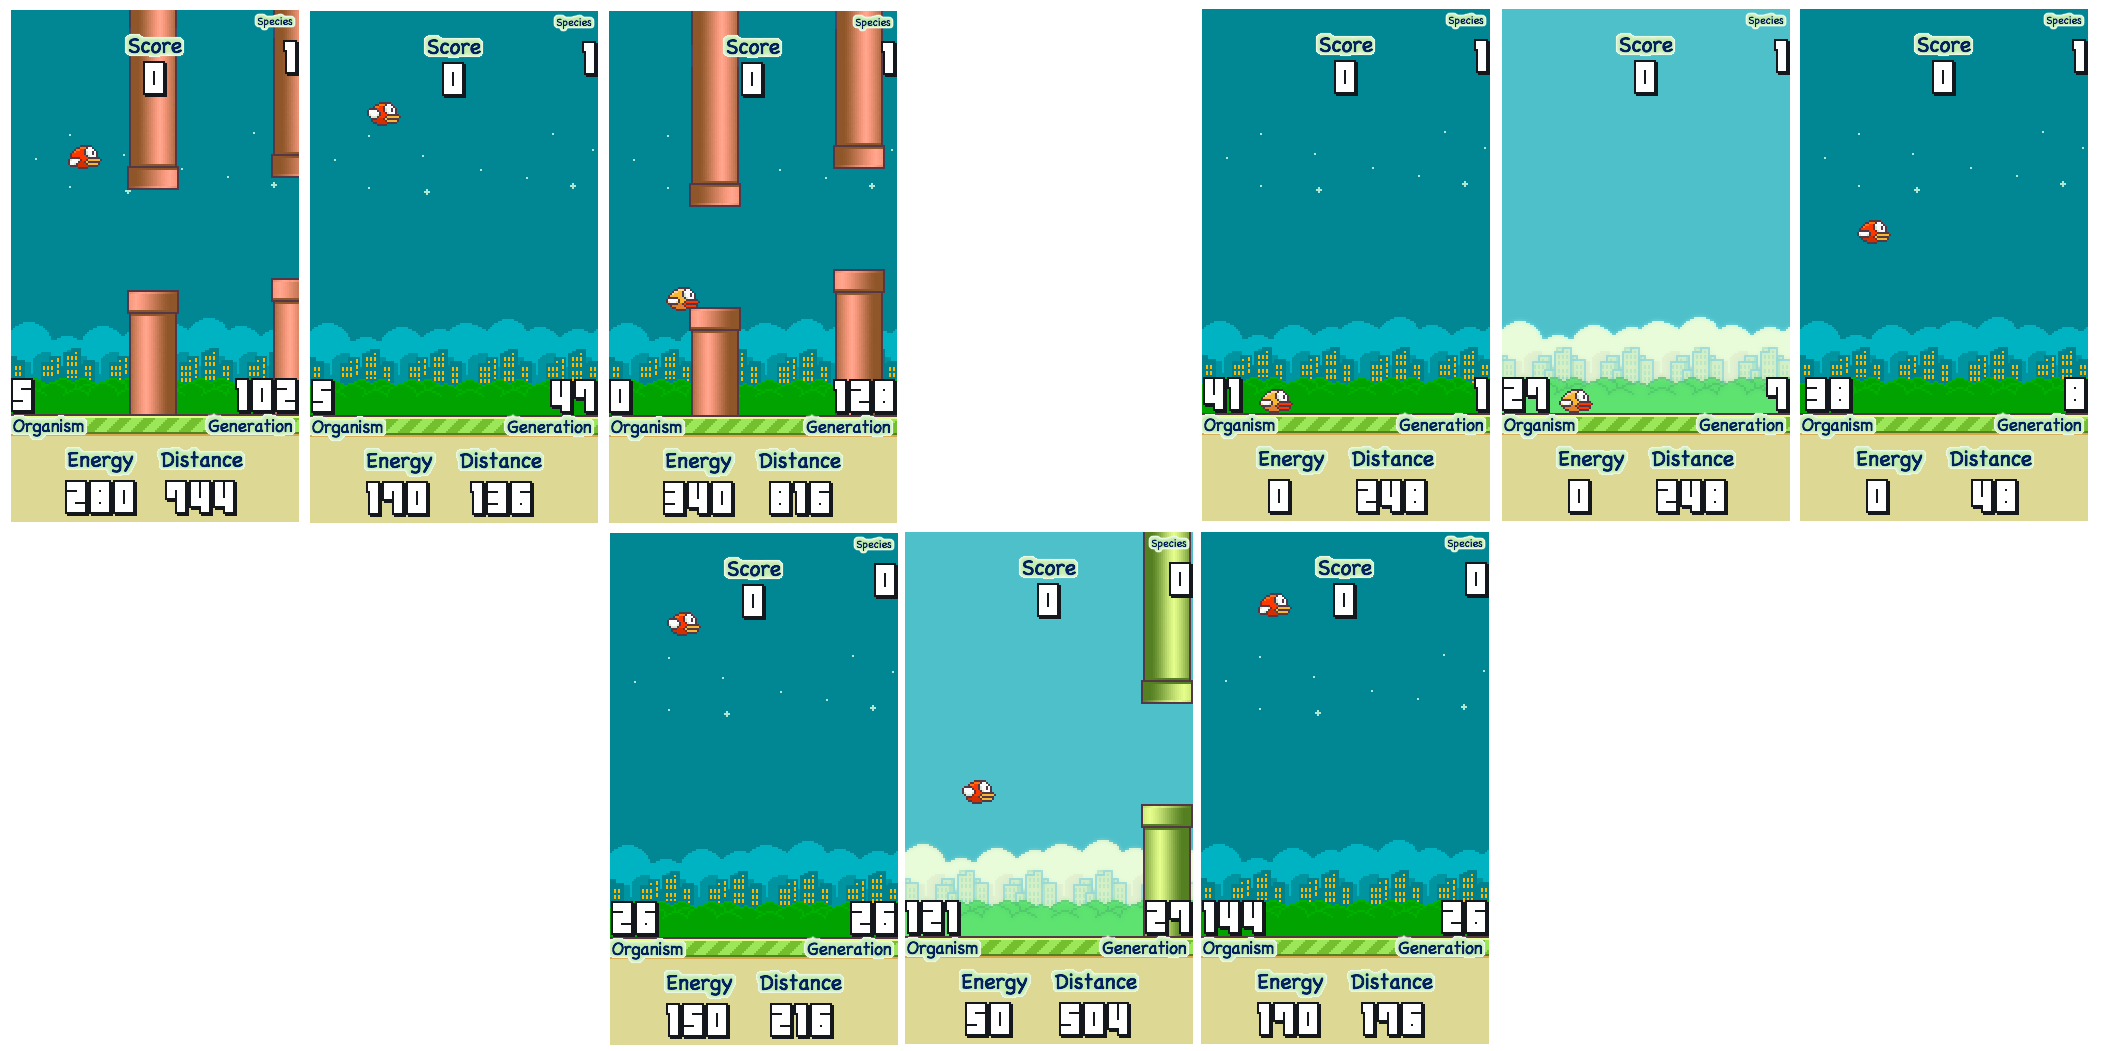
\includegraphics[width=1\textwidth]{graphics/flappy/flappy_sim_s1}
			\caption{Flappy Birds simulation}
		\end{figure}
		
		\begin{enumerate}
			\item explanation of environment and expectations
			\item fitnessfunction, formlar?
			\item explanation of graph of population (10, 50, 250) averaged on generations (30 generations evenly choosen [equal spaces between generation numbers])  (abstract explanation)
			\item check if expectations of marI/O can confirm
			\item huge difference between best runs and majority of runs (extreme luck), => double graph
			\item Differences between runs 
			\item unexpectedly bad results
			\item => Neat vs other machine learning
			\begin{enumerate}
				\item Differences between runs (lucky runs with 4th champion generation)
			\end{enumerate}
		\end{enumerate}
		
		\paragraph{Population 10 / Generation 500}
			asdf
%			\begin{figure}[h!]
%				\centering
%				\begin{minipage}{0.33\textwidth}
%					\centering
%					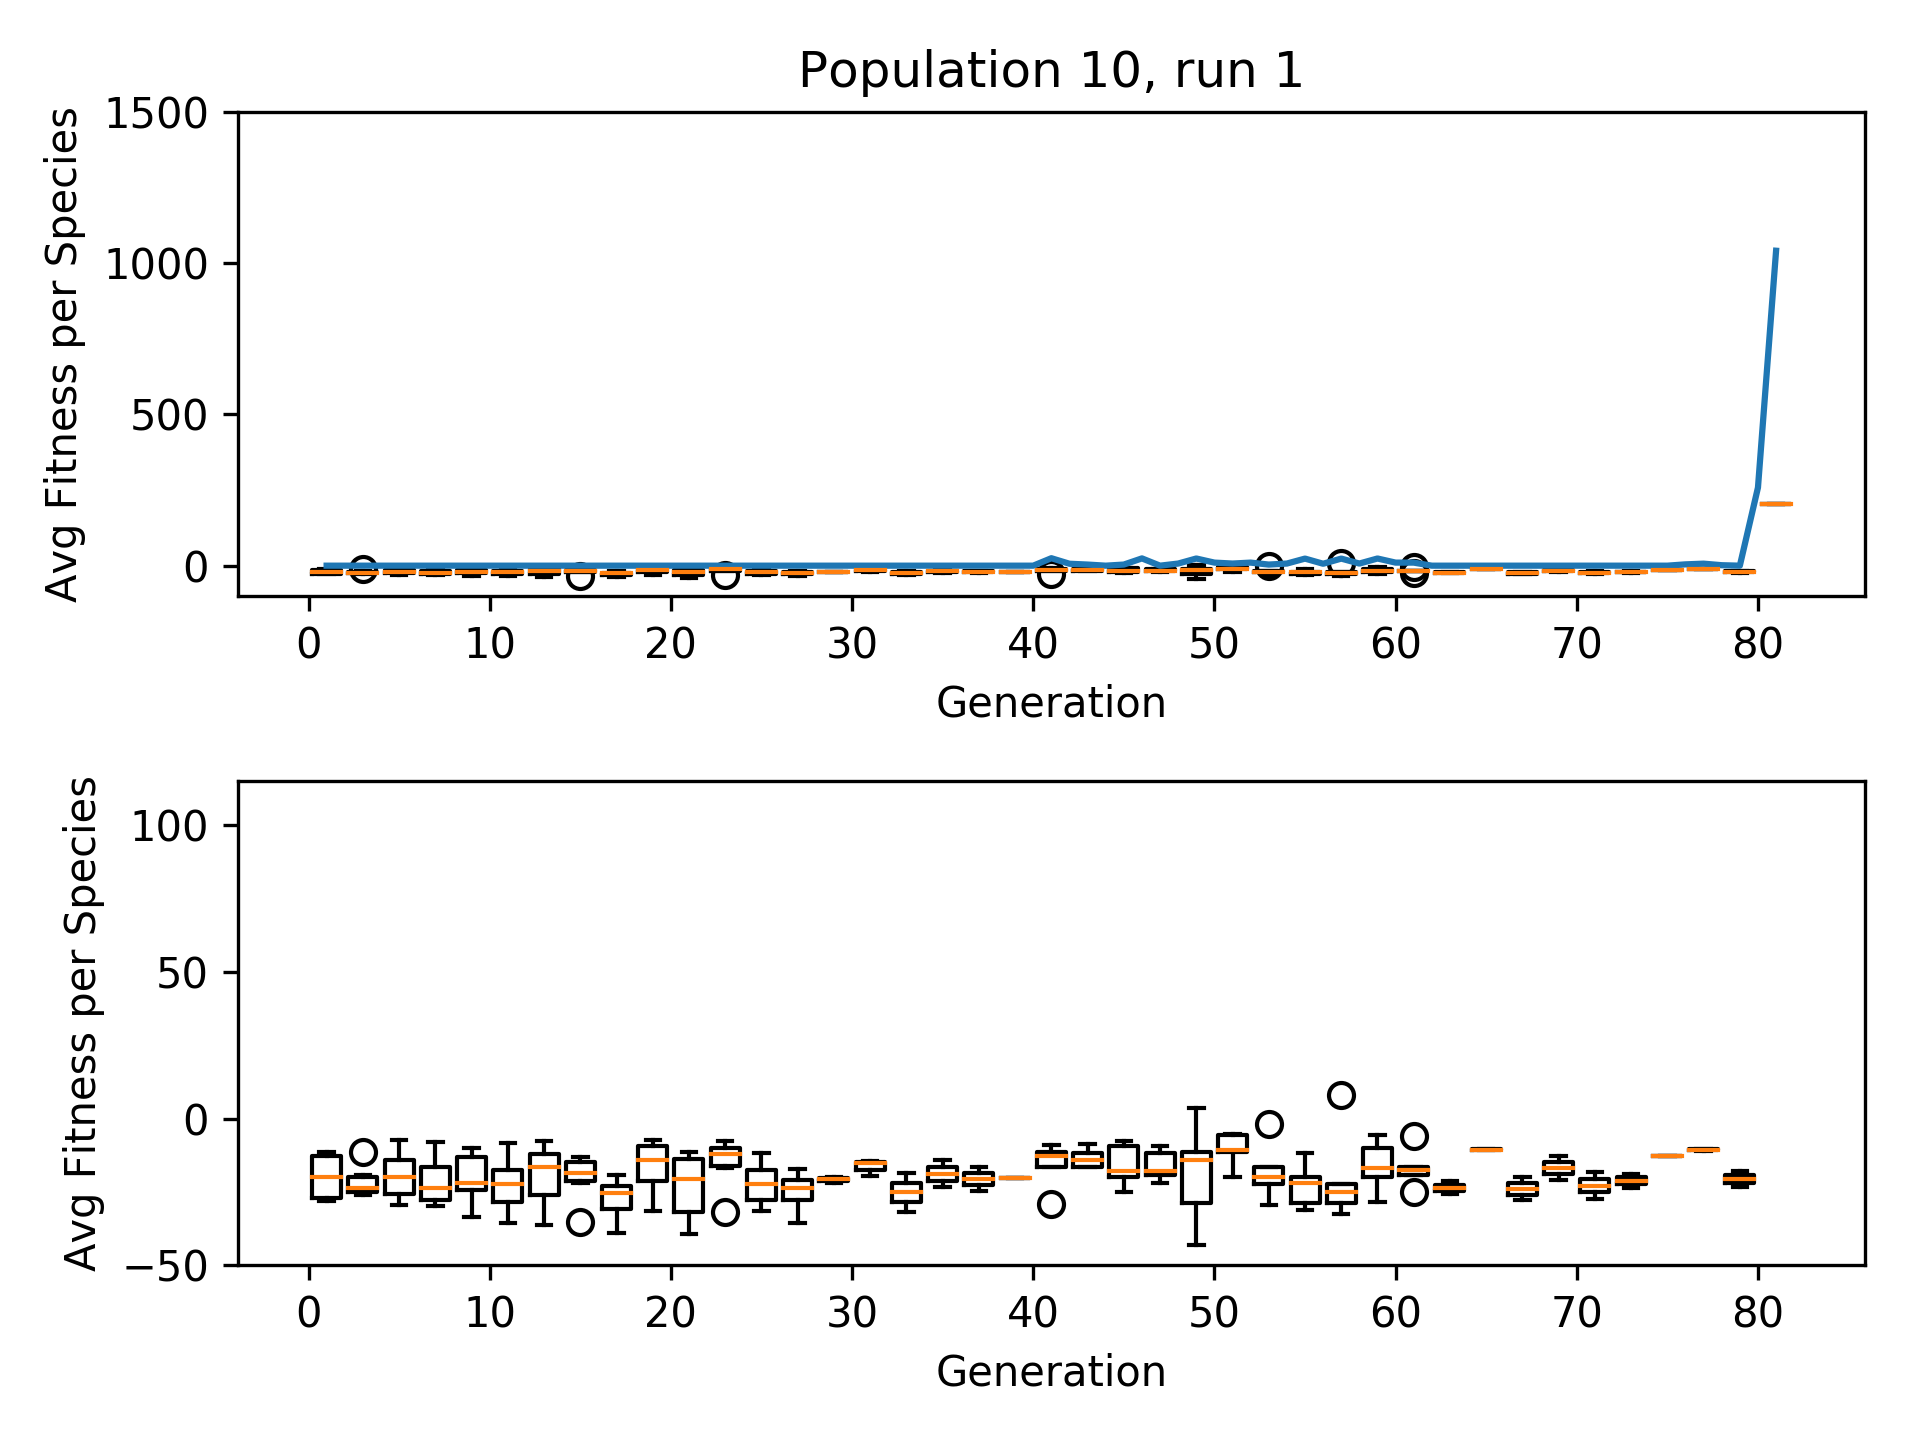
\includegraphics[width=1\textwidth]{graphics/flappy/pop10_run1} % first figure itself
%				\end{minipage}\hfill
%				\begin{minipage}{0.33\textwidth}
%					\centering
%					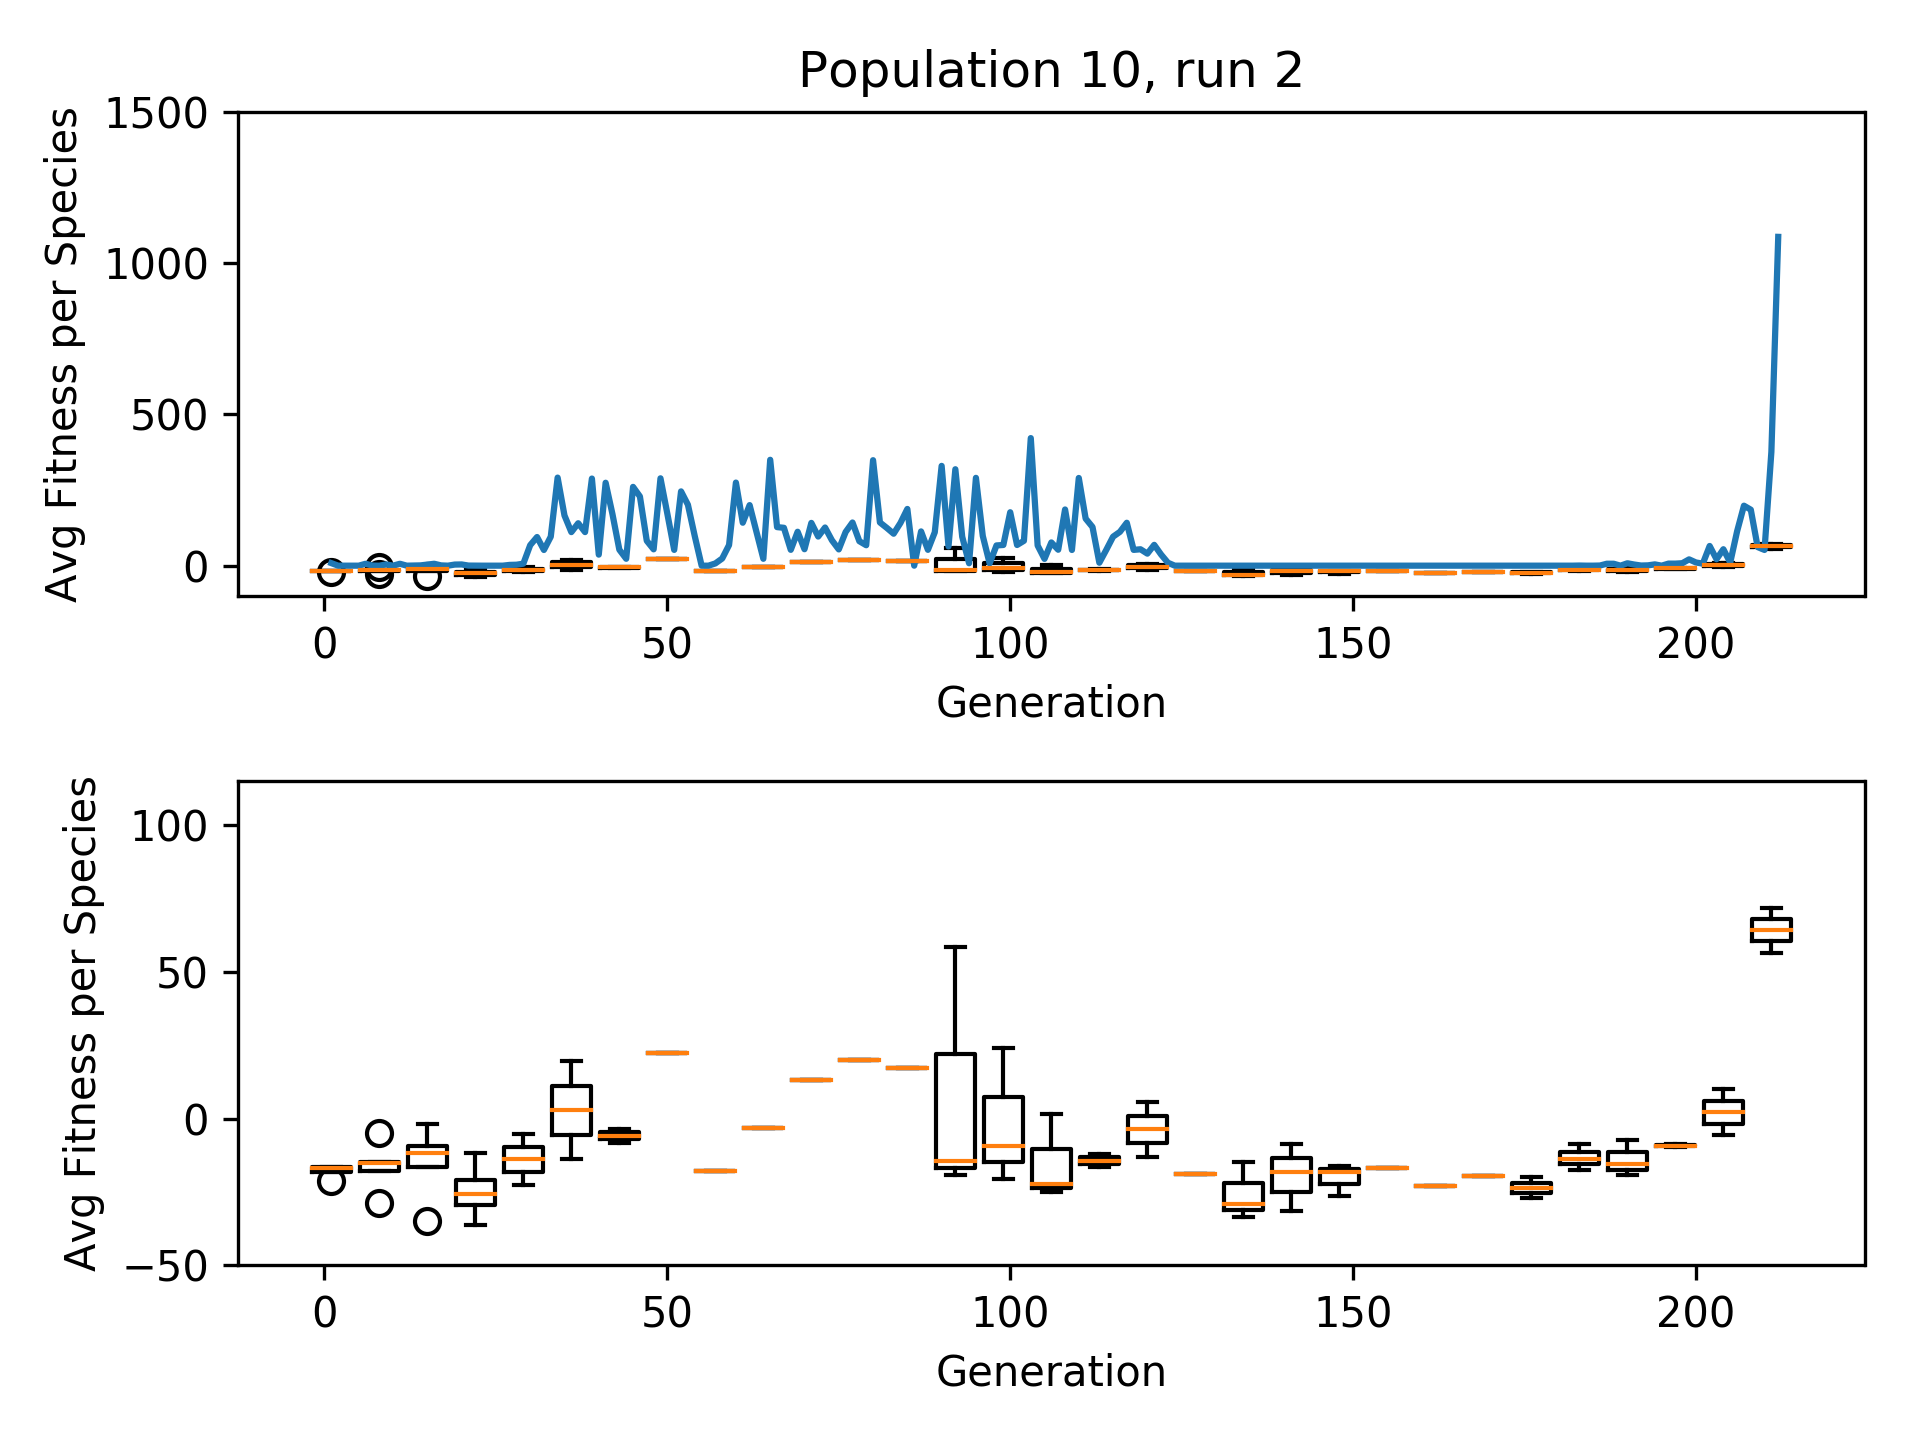
\includegraphics[width=1\textwidth]{graphics/flappy/pop10_run2} % second figure itself
%				\end{minipage}
%				\begin{minipage}{0.33\textwidth}
%					\centering
%					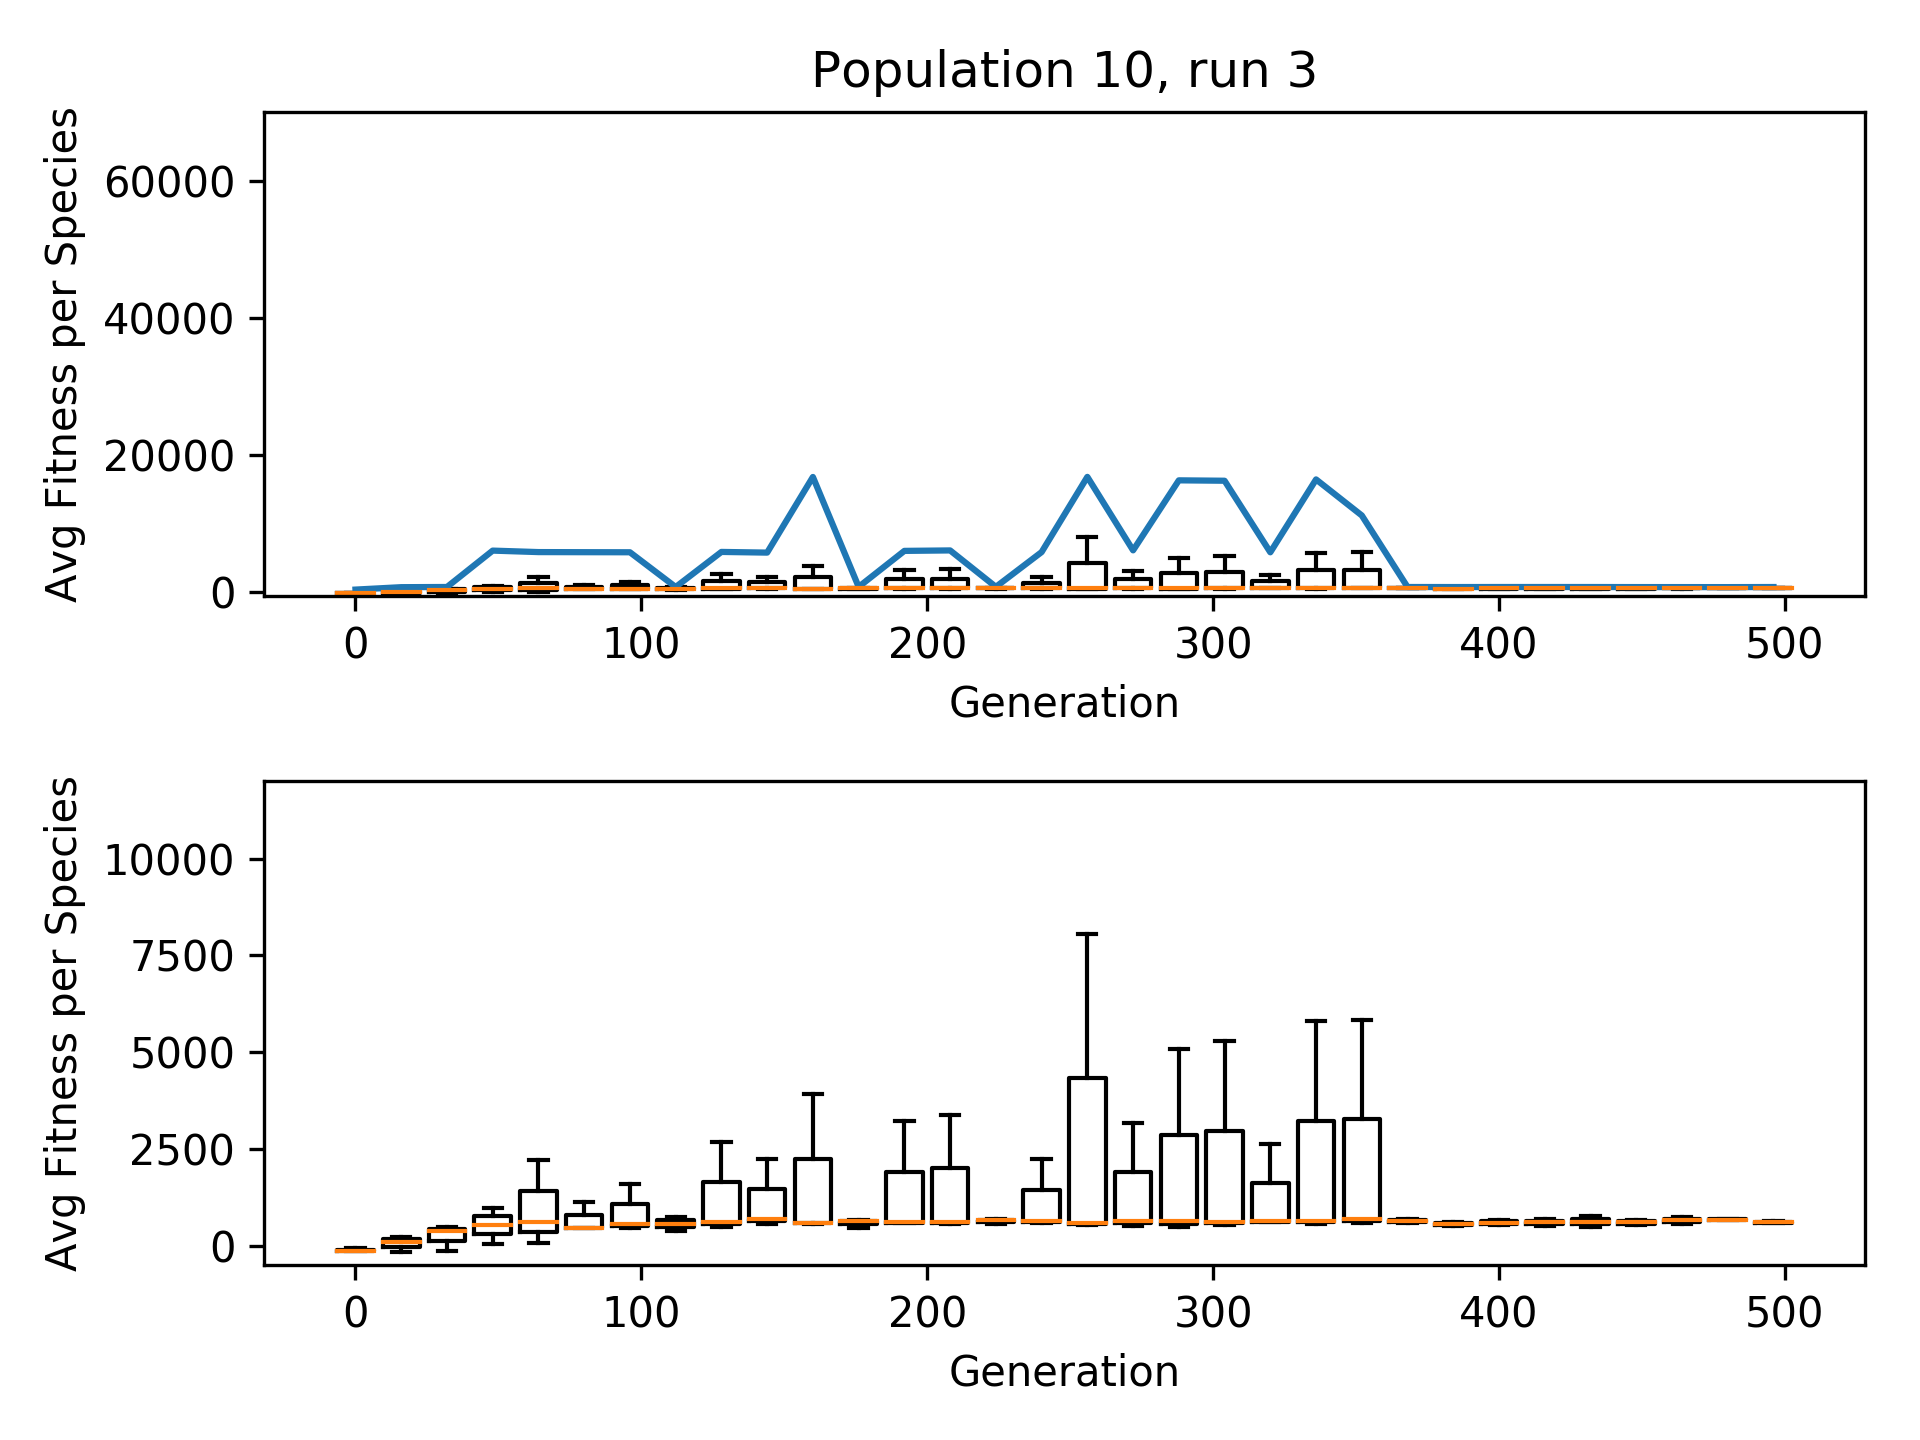
\includegraphics[width=1\textwidth]{graphics/flappy/pop10_run3} % second figure itself
%				\end{minipage}
%				\caption{Flappy Bird Population 10}
%			\end{figure}
		
		\paragraph{Population 50 / Generation 100}
			a
%			\begin{figure}[h]
%				\centering
%				\begin{minipage}{0.33\textwidth}
%					\centering
%					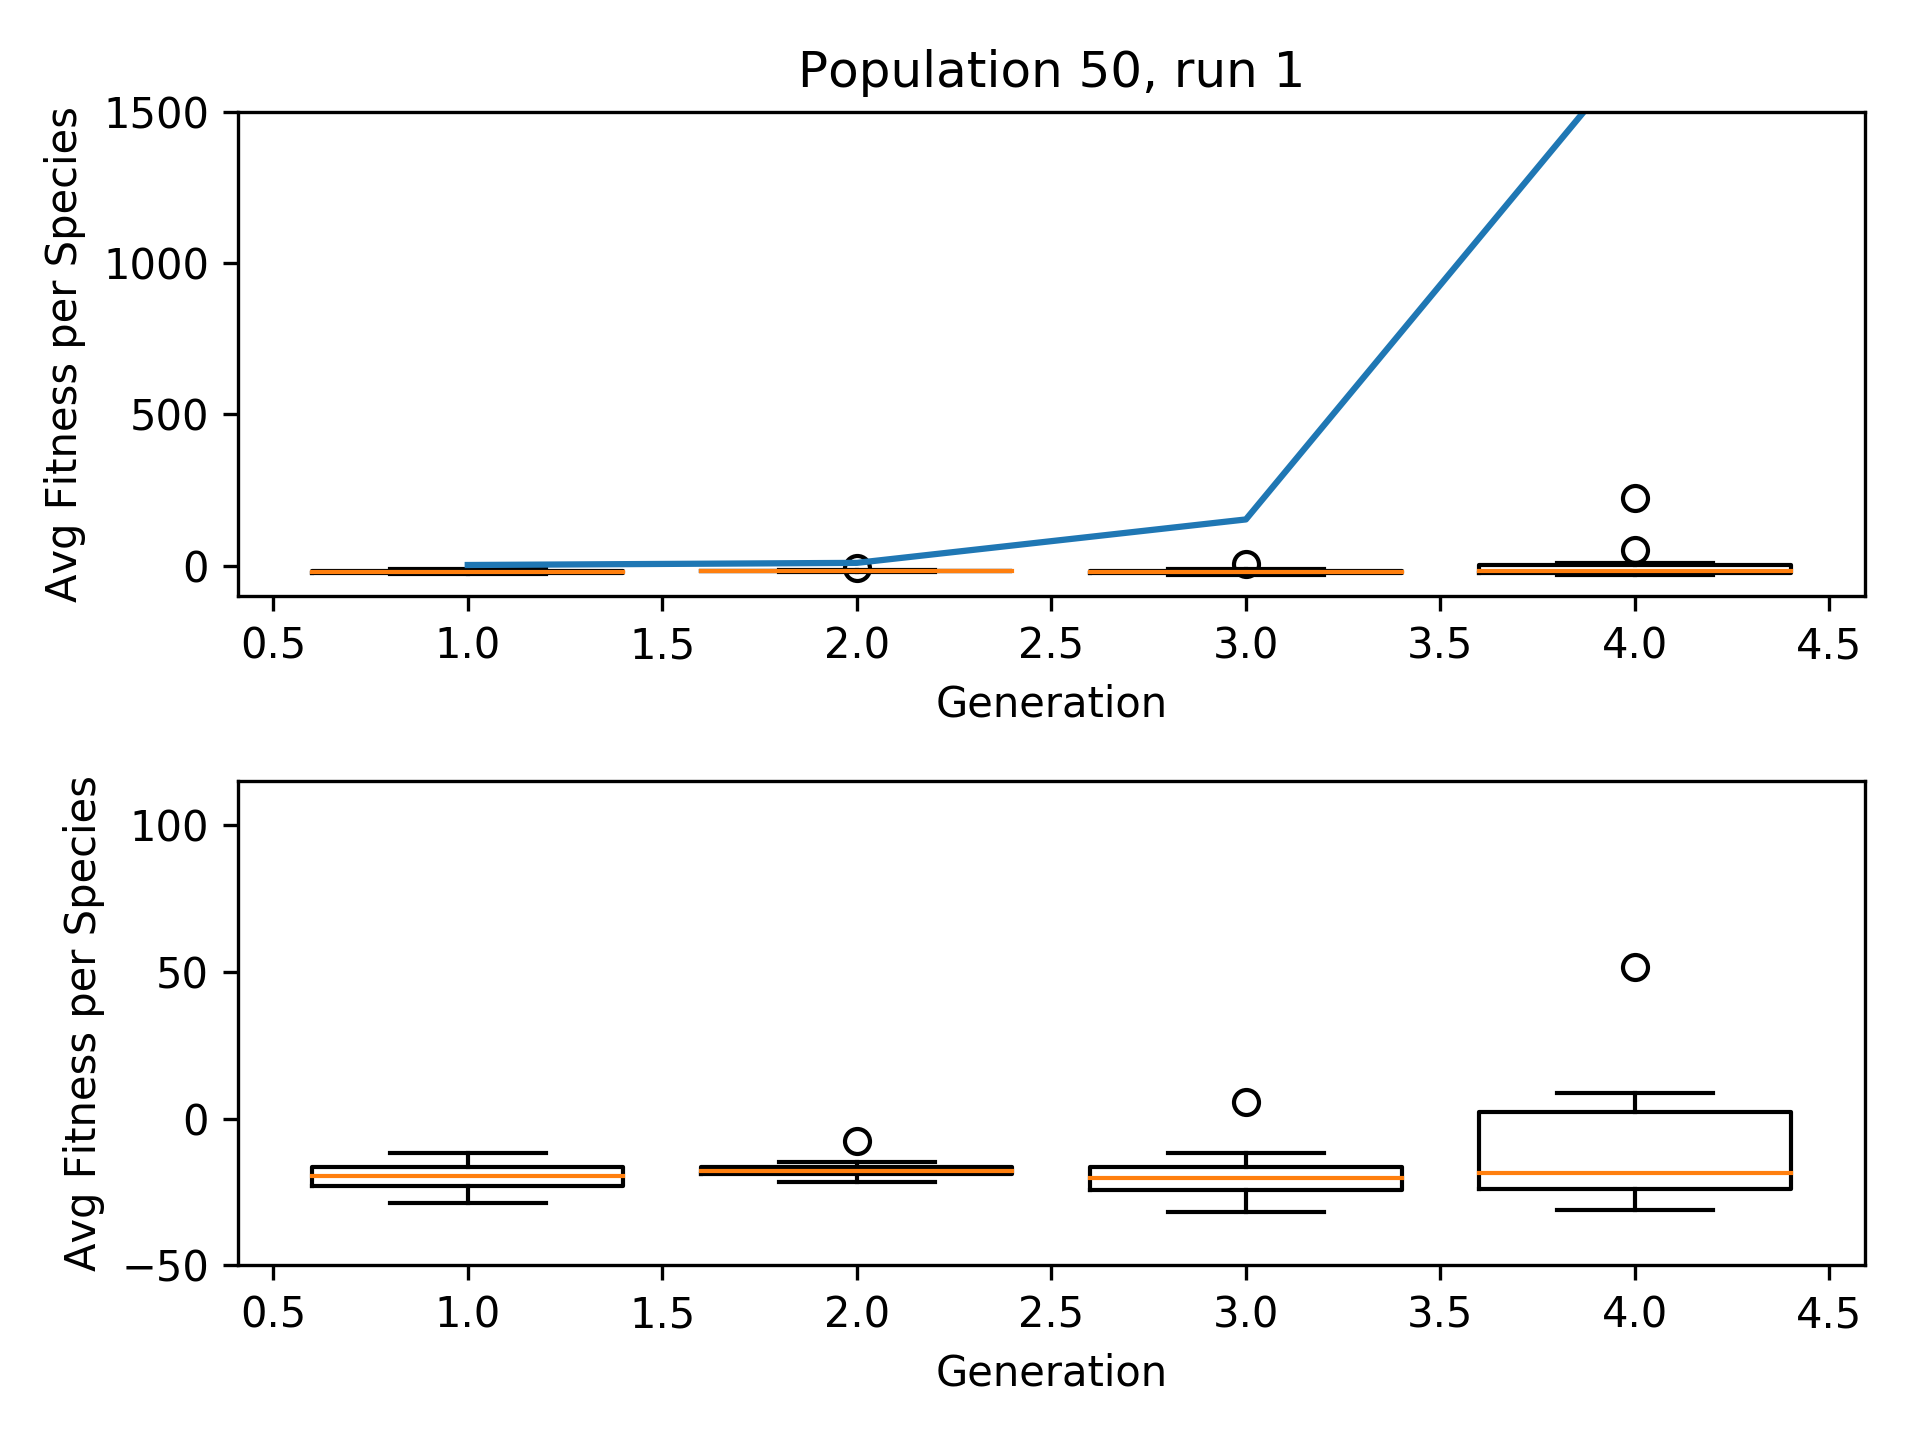
\includegraphics[width=1\textwidth]{graphics/flappy/pop50_run1} % first figure itself
%				\end{minipage}\hfill
%				\begin{minipage}{0.33\textwidth}
%					\centering
%					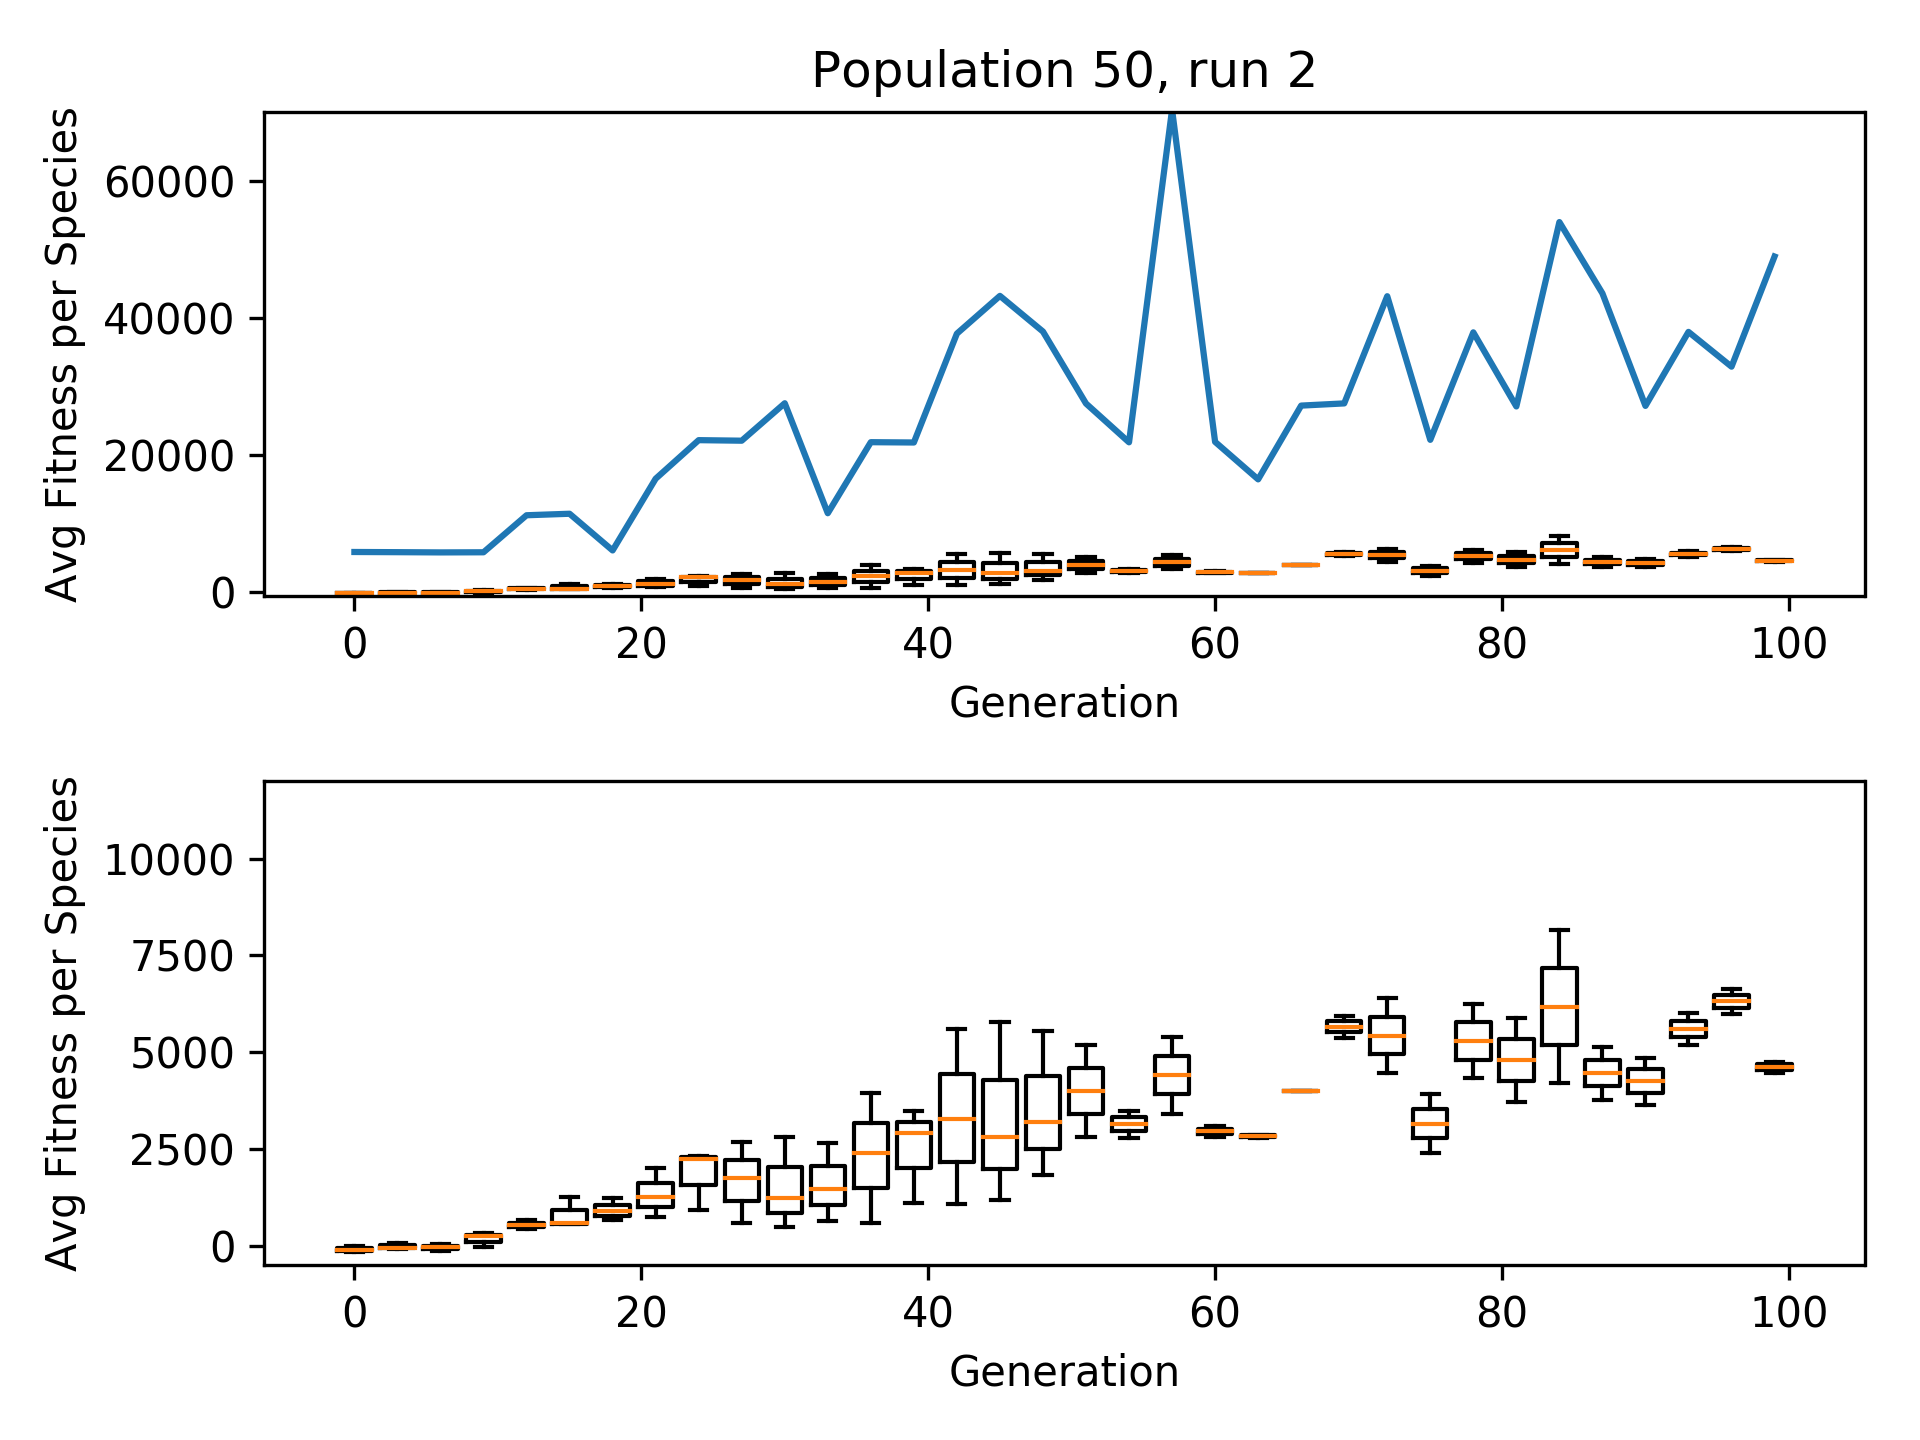
\includegraphics[width=1\textwidth]{graphics/flappy/pop50_run2} % second figure itself
%				\end{minipage}
%				\begin{minipage}{0.33\textwidth}
%					\centering
%					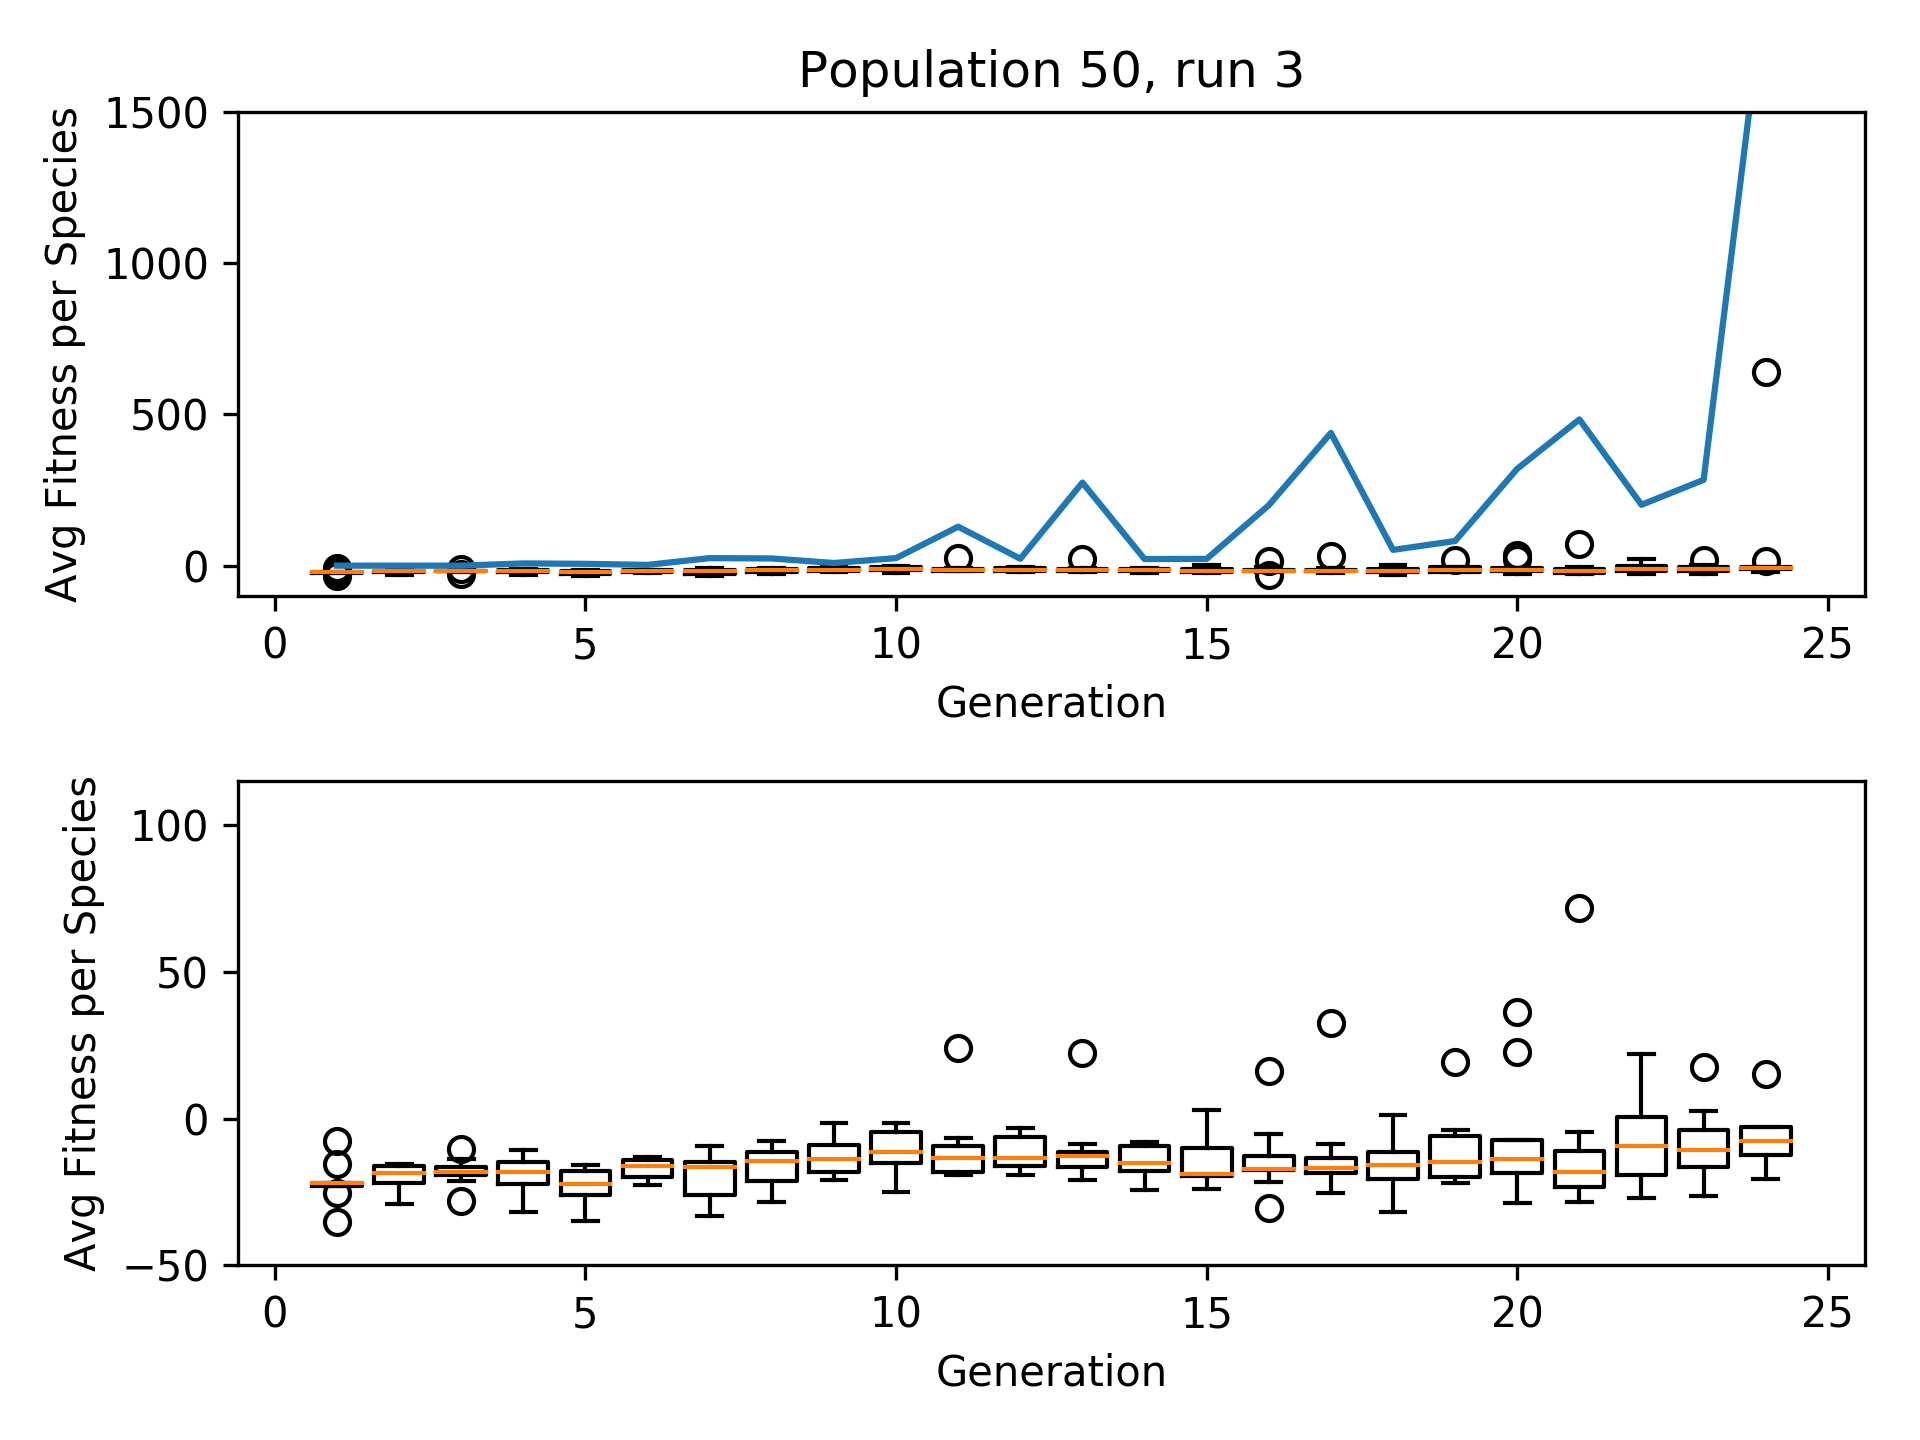
\includegraphics[width=1\textwidth]{graphics/flappy/pop50_run3} % second figure itself
%				\end{minipage}
%				\caption{Flappy Bird Population 50}
%			\end{figure}
		
		\paragraph{Population 250 / Generation 30}
		
			\begin{enumerate}
				\item best runs are exceptions (outside of whiskers)
			\end{enumerate}
			
%			\begin{figure}[h]
%				\centering
%				\begin{minipage}{0.33\textwidth}
%					\centering
%					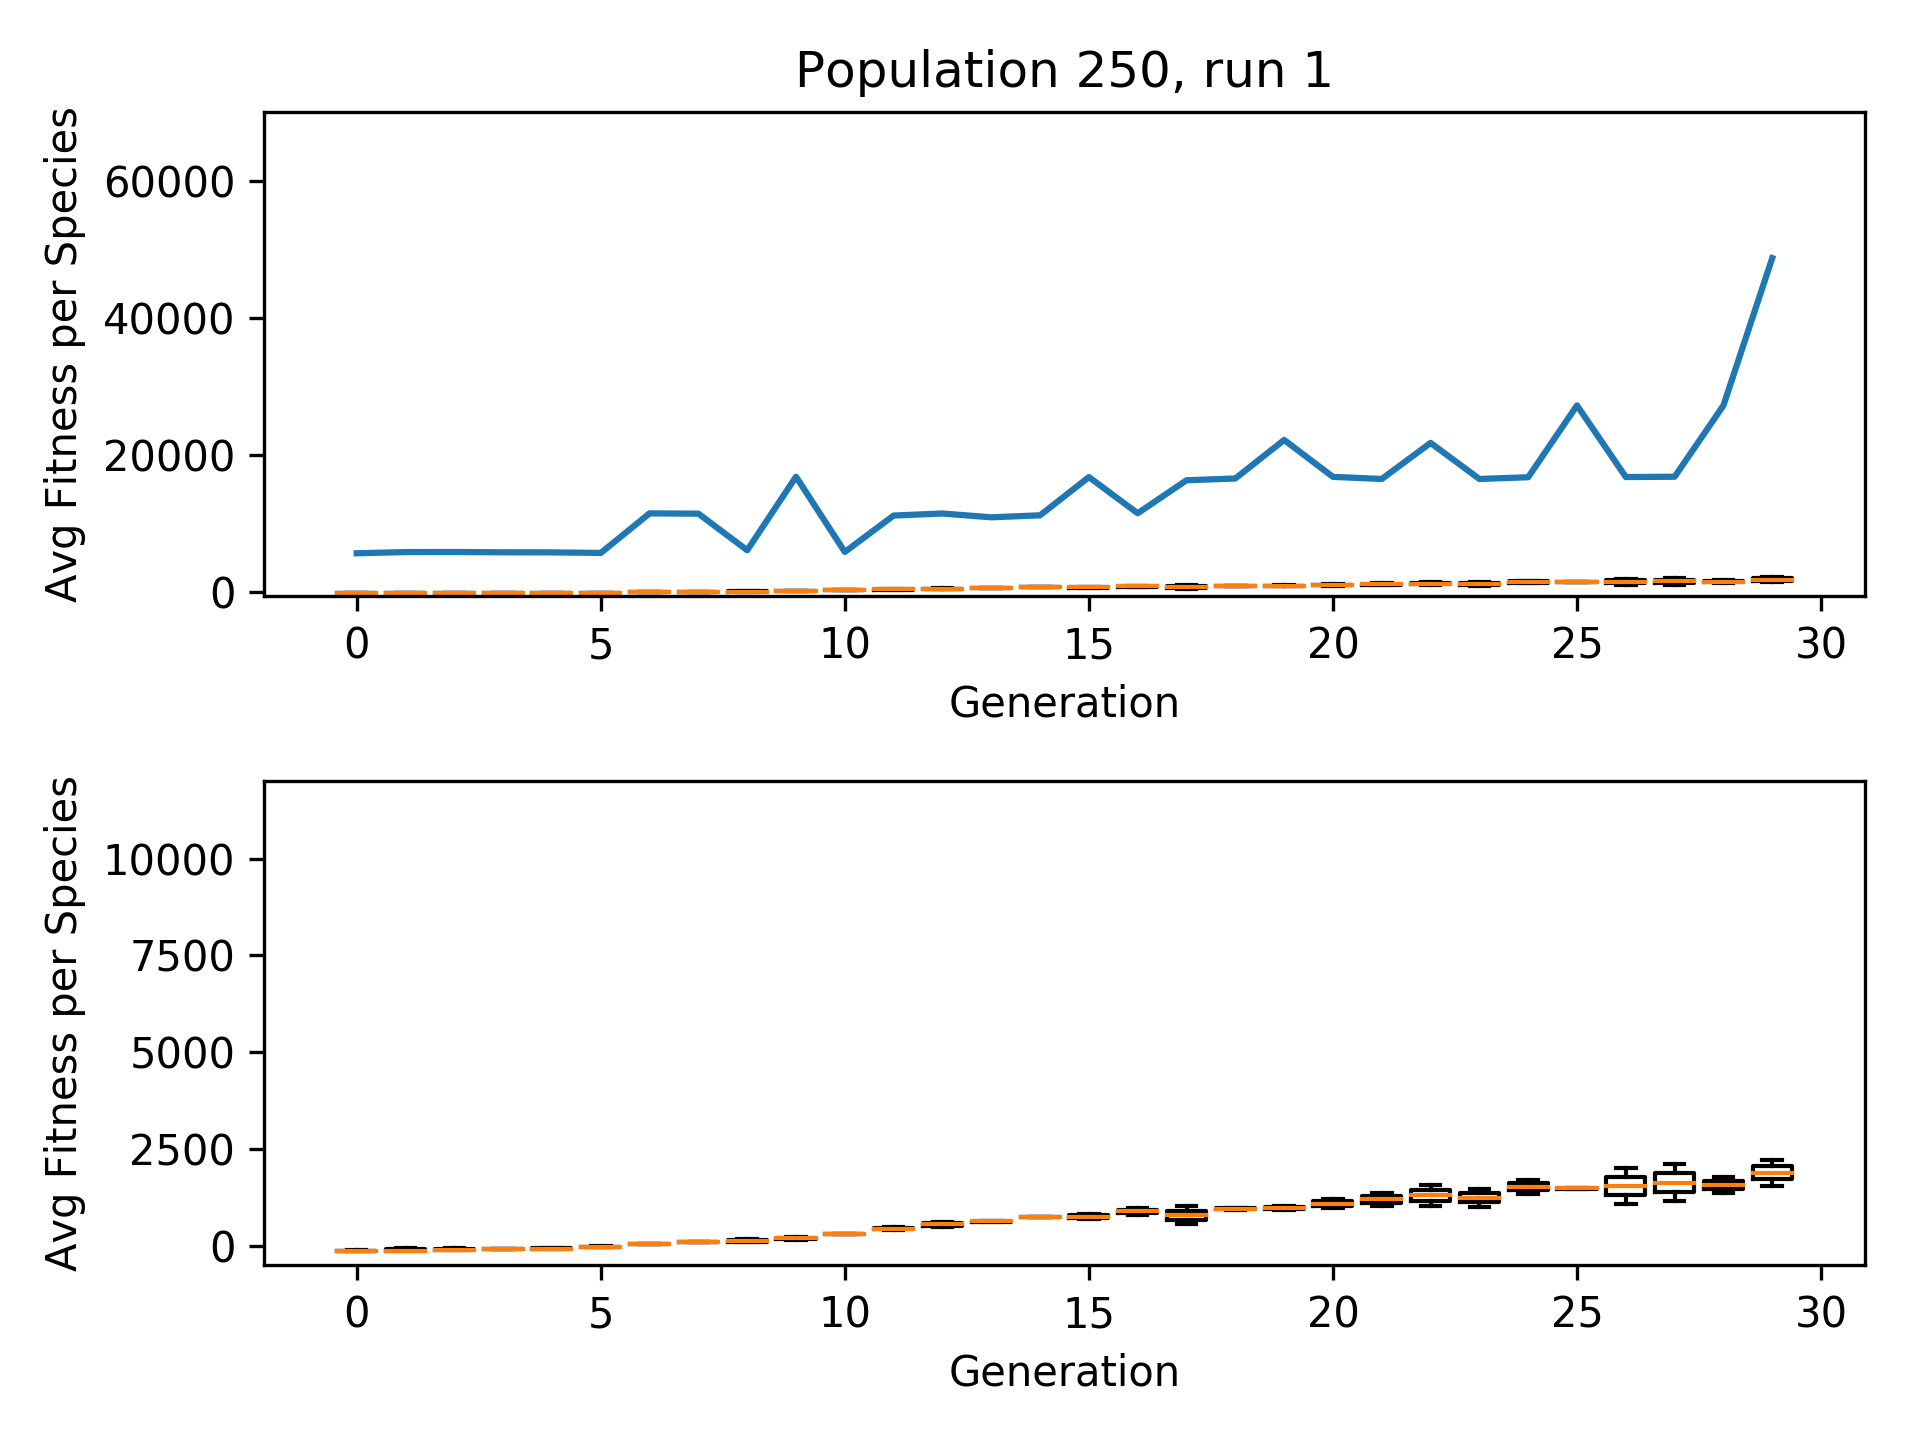
\includegraphics[width=1\textwidth]{graphics/flappy/pop250_run1} % first figure itself
%				\end{minipage}\hfill
%				\begin{minipage}{0.33\textwidth}
%					\centering
%					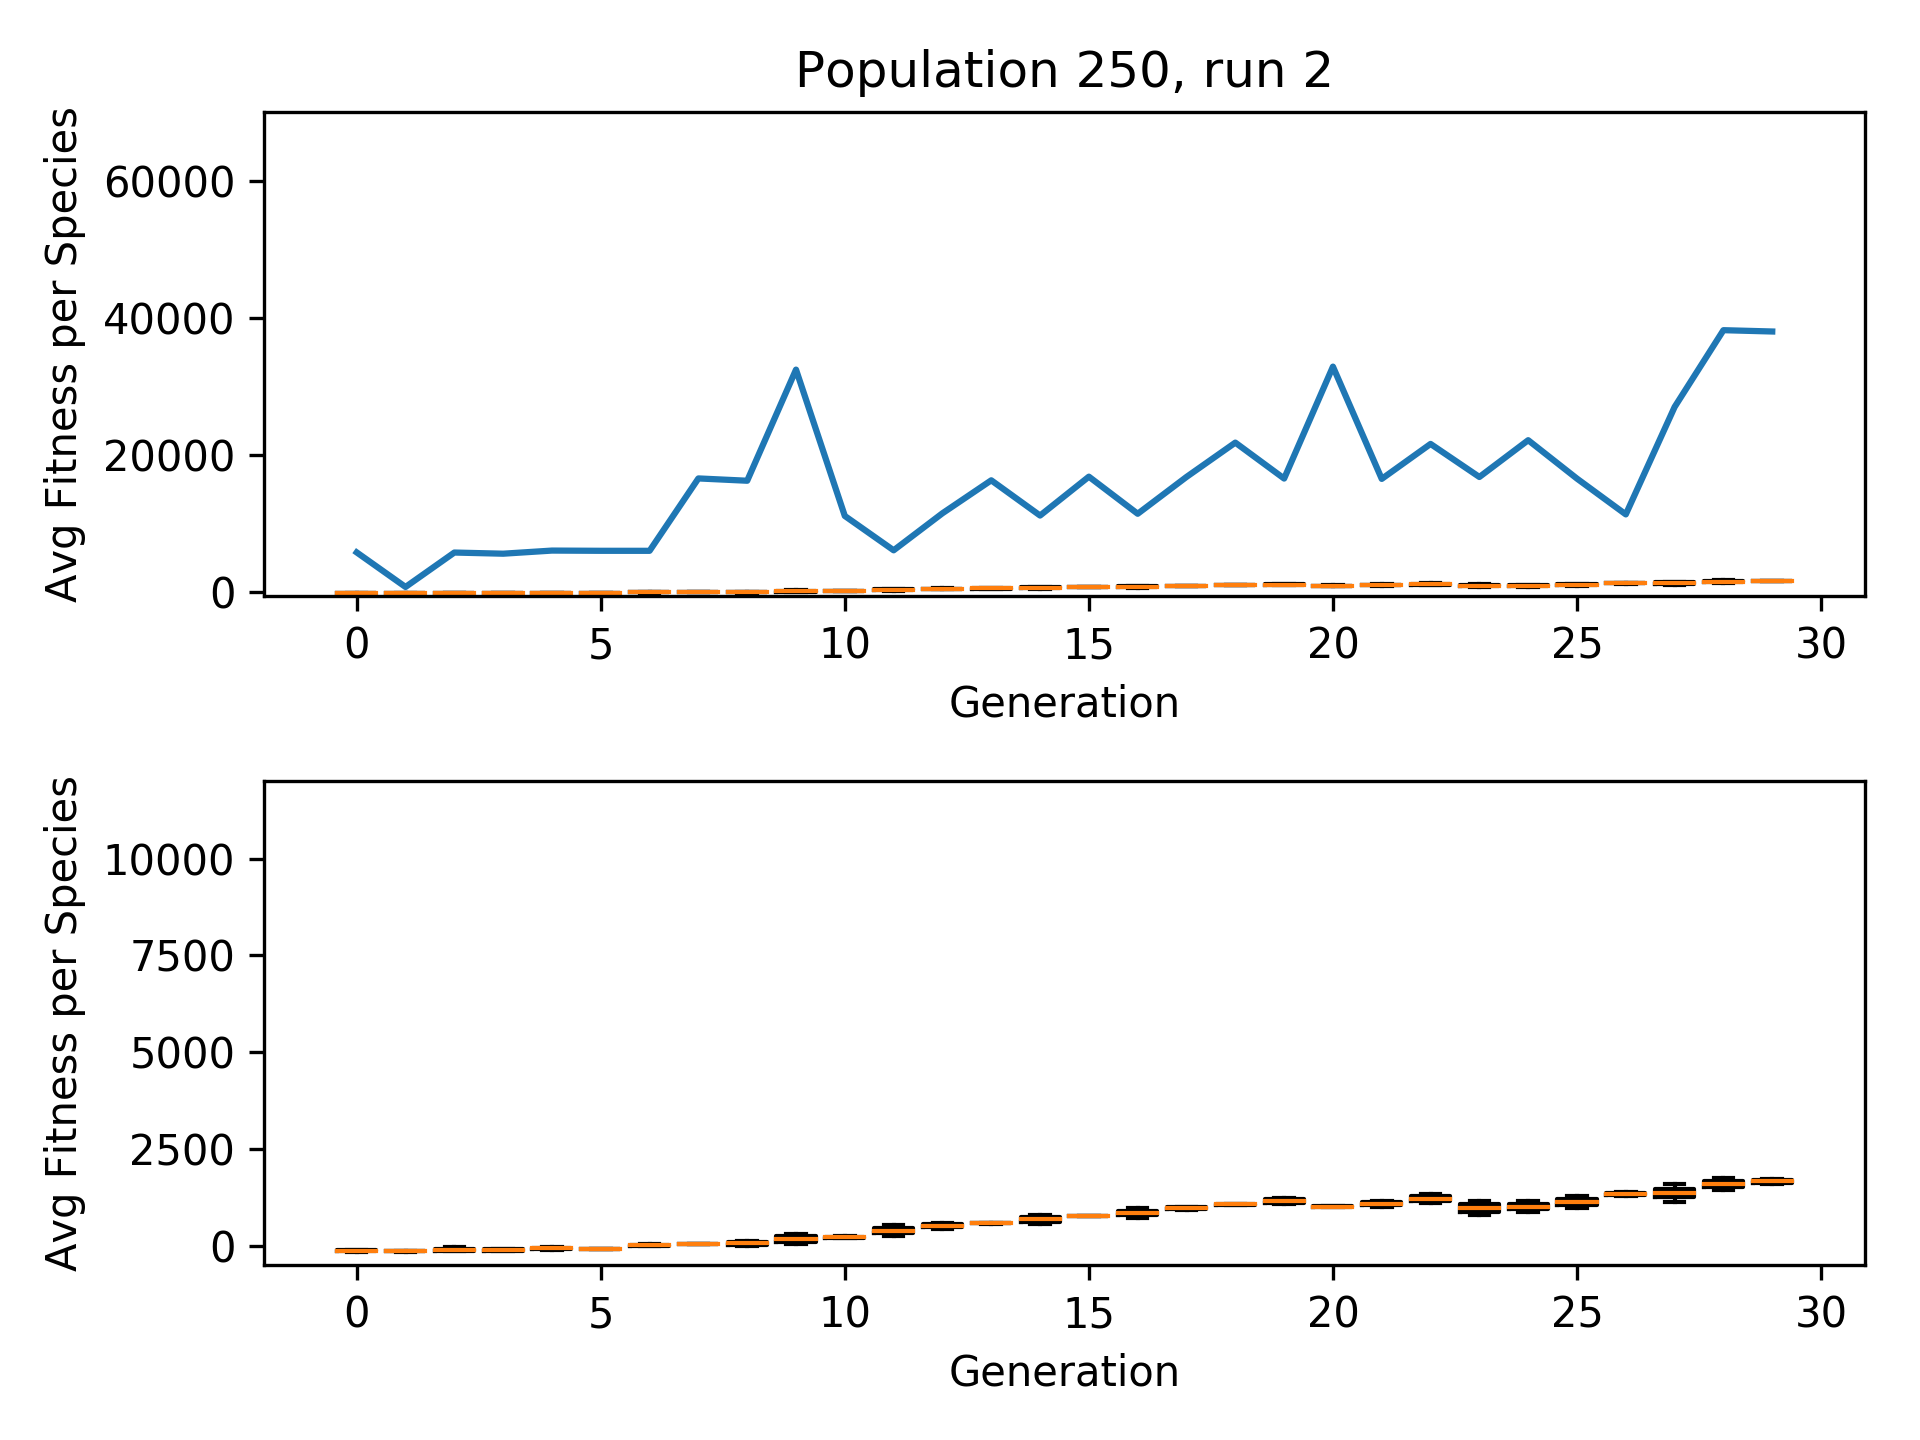
\includegraphics[width=1\textwidth]{graphics/flappy/pop250_run2} % second figure itself
%				\end{minipage}
%				\begin{minipage}{0.33\textwidth}
%					\centering
%					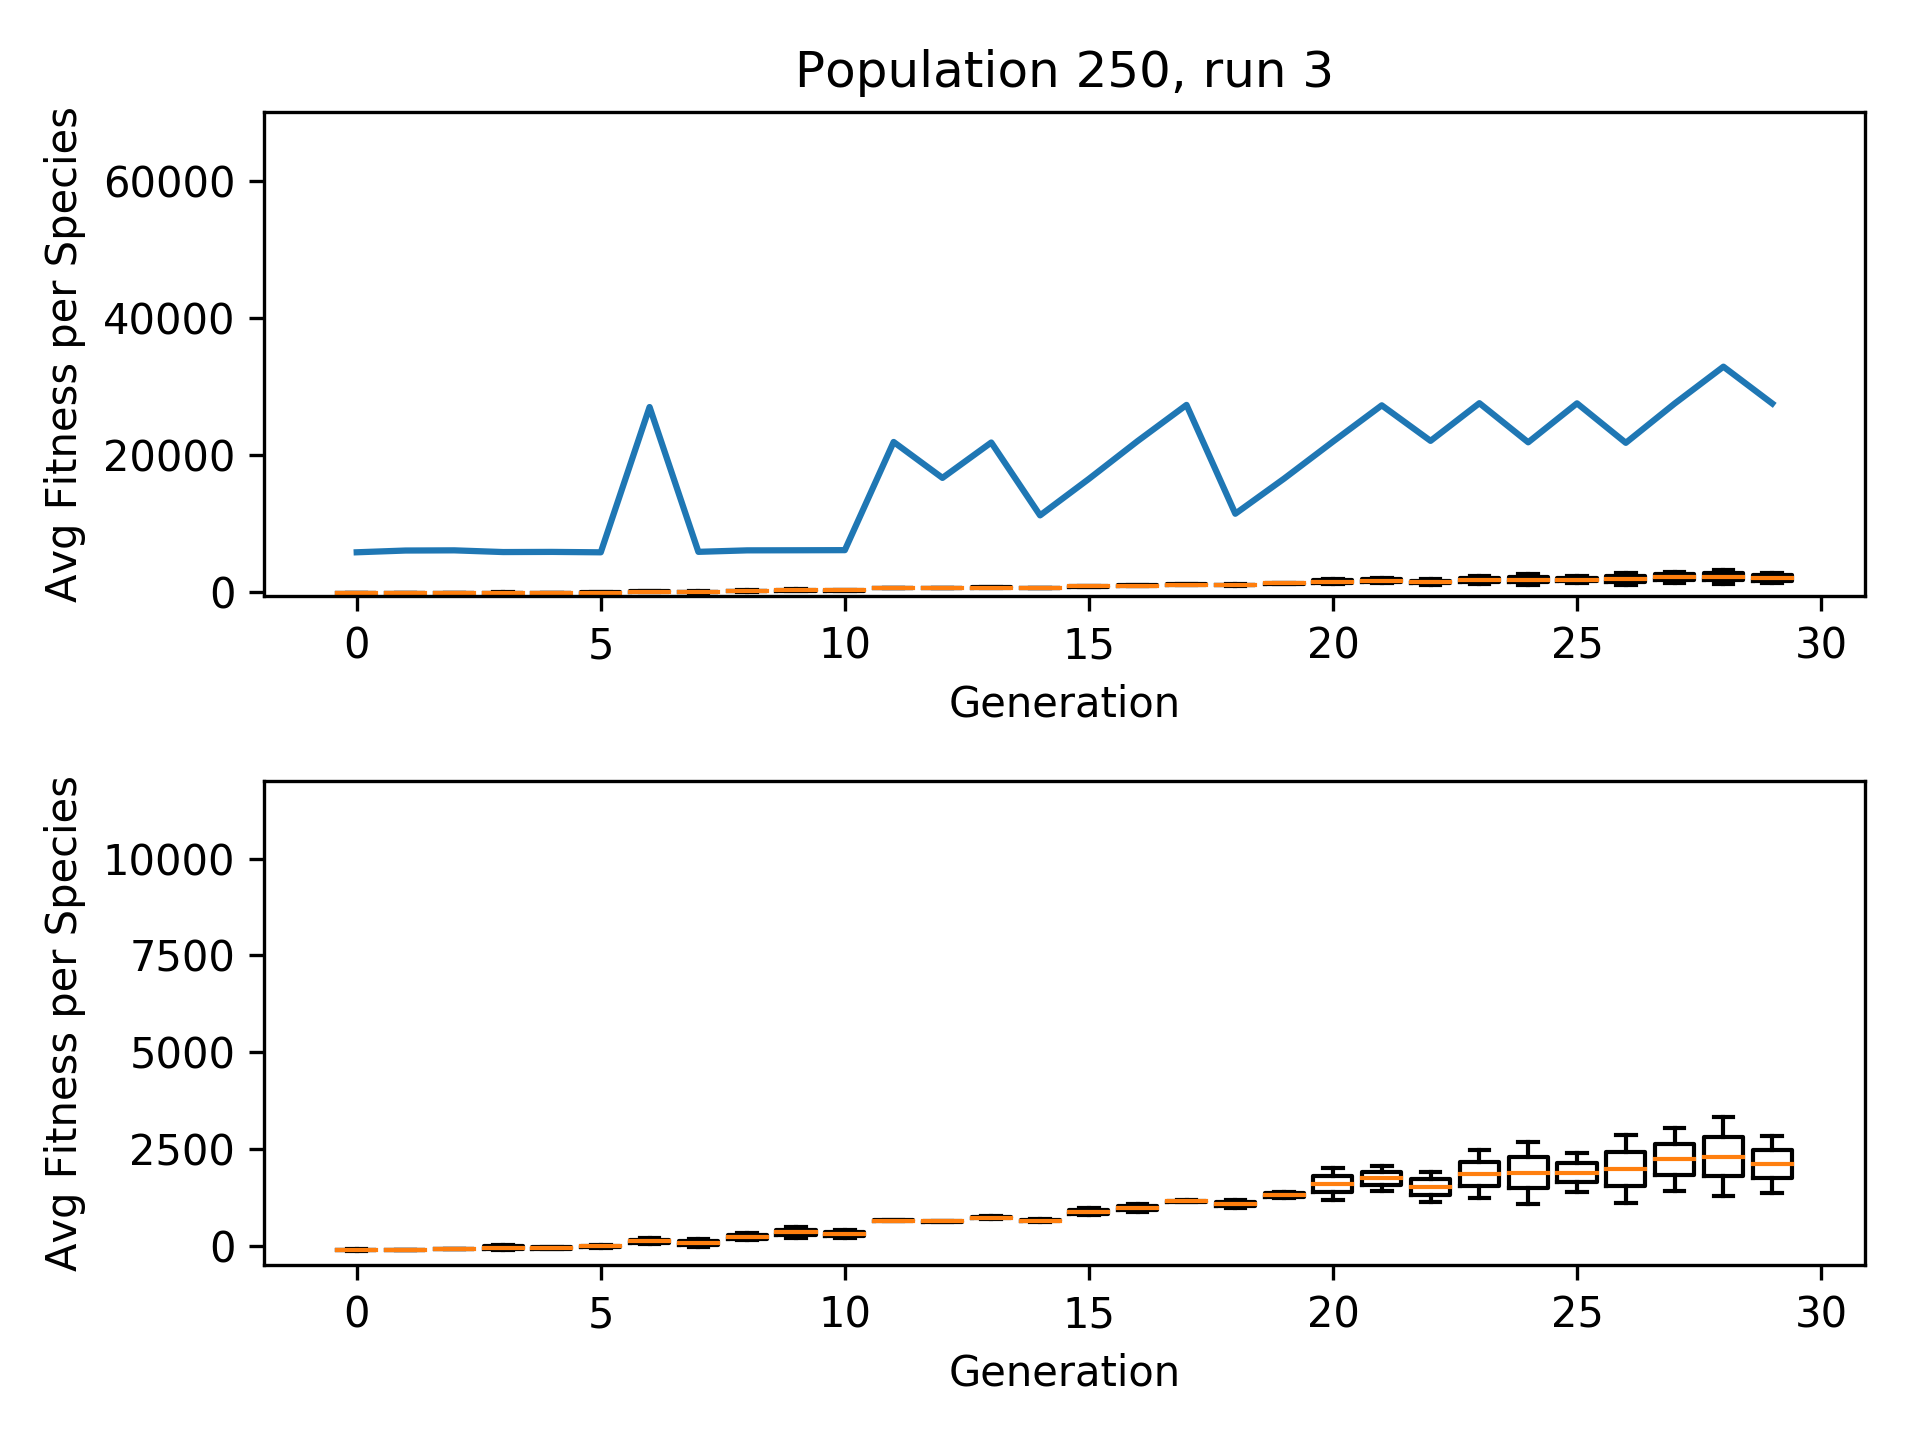
\includegraphics[width=1\textwidth]{graphics/flappy/pop250_run3} % second figure itself
%				\end{minipage}
%				\caption{Flappy Bird Population 250}
%			\end{figure}
		
		
		\subsection{Plain Machine learning flappy bird}
			\begin{enumerate}
				\item better results
				\item multi simulation made it easier
				\item easy algorithm for easy environment might be explanation for better results
			\end{enumerate}
	
	
	\section{Conclusion}
		\label{sec:system:conclusion}
		\begin{enumerate}
			\item differences / similarities in implementation (fixed size in machine learning flappy bird whereas dynamic species with marI/O)
			\item differences / similarities in outcome
			\item future studies
				\begin{itemize}
					\item genome/generation plot \& differences to other plot
					\item check in text for (future or further)
				\end{itemize}
		\end{enumerate}

